%\chapter{Love and Rayleigh Waves}
\chapter{勒夫波与瑞利波}
\label{chapter:surfacewaves}

到目前为止,在本书中我们已经将地球对地震震源的响应表示为正交归一的自由振荡或{\em 驻波\/}的叠加。
我们也可以将该响应分解为{\em 行波\/}的叠加。
\index{standing wave}%
\index{travelling wave}%
在球面上将驻波表达式转换为行波表达式是一个经典的分析方法,它适用于声波或电磁波,也适用于弹性波。该方法的数学基础是所谓的{\em Watson变换\/},我们将在第~\ref{sec.11.Watson}节中介绍。
其后我们在第~\ref{sec.11.Green}和~\ref{sec.11.resp}节中对该变换在地震学的应用,是对~\textcite{gilbert76a}、\textcite{dahlen79}和 ~\textcite{snieder&nolet87}的工作的延伸,同时也为分析体波和面波提供了一个统一的处理方法。

当实现了从模式叠加响应到行波表达式的在弱非弹性球对称地球上一致有效的变换之后,我们将在本章的剩余部分专门讨论勒夫和瑞利面波,它们分别等价于~$n\ll l/4$~的自由震荡多态模式~${}_n{\rm T}_l$~和~${}_n{\rm S}_l$。
这些围陷波的几何扩散局限于二维而非三维空间;因为如此,也由于它们受到浅源地震的强烈激发,在大多数地震图上基阶面波是振幅最大的讯号。
在一个给定的径向分支~$n=0,1,2,\ldots$~上,长周期的波比短周期的波 "感受"到地球更深部的弹性和密度结构;因此,勒夫和瑞利波的传播是有{\em 频散的\/}。
\index{dispersion!Rayleigh-wave}%
\index{dispersion!surface-wave}%
\index{surface-wave dispersion}%
\index{Rayleigh-wave dispersion}%
\index{Love-wave dispersion}%
\index{dispersion!Love wave}%
实际应用中,由于地壳和上地幔结构的地理差异,面波频散是有区域性变化的;我们在第~16~章中将会看到,本章中的大部分分析在~JWKB~近似的背景下完全适用于横向不均匀的地球。

%\section{Watson Transformation}
\section{Watson变换}
\index{Watson transformation|(}%
\index{transformation!Watson|(}%
\label{sec.11.Watson}

转换过程的第一步是将对球谐函数次数~$l$~的求和表示成对波数~$k$~的积分。
这是通过所谓的{\em Watson变换\/}来实现的:
\index{wavenumber}%
\eq
\sum_{l=0}^\infty f(l+\half)=\half\int_Cf(k)e^{-ik\pi}(\cos k\pi)^{-1}dk.
\label{eq:11.Watson}
\en
(\ref{eq:11.Watson})~这一等式对任何在实数~$k$~轴附近解析的函数~$f(k)$~都成立;
积分是沿着复数~$k$~平面上的闭合路径~$C$,如图~\ref{fig.watson}所示。
被积函数在正的半整数值~$k=1/2,\,3/2,\,5/2,\ldots$~处有简单极点,
因此上面的等式可以很容易地用由留数定理计算环路积分来验证。
\begin{figure}[!b]
\begin{center}
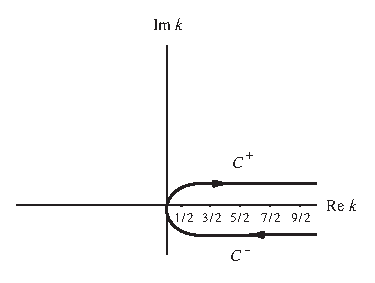
\includegraphics{../figures/chap11/fig01.eps}
\end{center}
\caption[Watson contour]{\label{fig.watson}
复数波数平面的示意图,图中显示~Watson~环路~$C=C_-+C_+$。
在简单极点~$k=l+1/2$~处的留数为~$i\pi^{-1}f(l+1/2)$。}
\end{figure}

对我们的目的而言,Watson变换的一个更有用的形式是{\em 泊松叠加公式\/},
\index{Poisson sum formula}%
我们下面来展示,它可以从~(\ref{eq:11.Watson})~式很容易地得到。
在积分环路位于~$k$~的下半平面的部分~$C^-$,我们有
\eq
(\cos k\pi)^{-1}=\frac{2e^{-ik\pi}}{1+e^{-2ik\pi}}
=-2\sum_{s=1}^\infty(-1)^se^{-i(2s-1)k\pi}.
\label{eq:11.sec1}
\en
由于在~$C^-$~上~$\Im{\rm m}\,k<0$,因此对~$s$~的求和是收敛的。
用类似的推论,在积分环路位于上半平面的部分~$C^+$~有
\eq
(\cos k\pi)^{-1}=\frac{2e^{ik\pi}}{1+e^{2ik\pi}}=
2\sum_{s=-\infty}^{0}(-1)^se^{-i(2s-1)k\pi}.
\label{eq:11.sec2}
\en
将~(\ref{eq:11.sec1})~和~(\ref{eq:11.sec2})~式合并,我们可以将变换~(\ref{eq:11.Watson})~改写为
\eq
\sum_{l=0}^\infty f(l+\half)=\sum_{s=-\infty}^\infty(-1)^s
\int_0^\infty f(k)e^{-2isk\pi}\,dk,
\label{eq:11.Poisson}
\en
这里要记住,在~$s\rightarrow\infty$~的极限下,积分路径在实数~$k$~轴{\em 下面\/}从原点到~$\infty-i0$,而在~$s\rightarrow -\infty$~极限下,则在实数~$k$~轴{\em 上面\/}从原点到~$\infty+i0$。
当角标~$s$~的数值为有限时,路径的精确位置并不重要。
在下面的三节当中,我们将利用~(\ref{eq:11.Poisson})~这一等式来推出球对称地球的格林函数张量和地震的加速度响应的行波表达式。
\index{Watson transformation|)}%
\index{transformation!Watson|)}%

%\section{Travelling-Wave Decomposition}
\section{行波分解}
\index{travelling wave|(}%
\label{sec.11.Green}

稍微改变一下第~10.2~节中所使用的符号,我们将球对称地球格林函数张量的傅里叶变换
\eq \label{11.FTG}
\bG(\bx,\bx';\omega)=\int_0^{\infty}\bG(\bx,\bx';t)e^{-i\omega t}\,dt
\en
写为如下形式
\eq
\bG=\frac{1}{2\pi}\sum_{n=0}^\infty\sum_{l=0}^\infty
(l+\half)\,{}_{n\!}\bG_l\,P_l(\cos\Theta),
\label{eq:11.form}
\en
其中
\eq \label{11.form2}
{}_{n\!}\bG_l={}_n\bD_l
\left[\frac{\half(i\hspace{0.4 mm}{}_n\om_l)^{-1}}{\gammanl+i(\om-{}_n\om_l)}
+\frac{\half(-i\hspace{0.4 mm}{}_n\om_l)^{-1}}{\gammanl+i(\om+{}_n\om_l)}\right]
{}_n\bD_l^{\prime}.
\en
(\ref{11.form2})~式精确到固有品质因子倒数~$Q_{\kappa}^{-1}$~和~$Q_{\mu}^{-1}$~的一阶。
上式中除了洛伦兹谱峰~$\half[\gammanl+i(\om\pm{}_n\om_l)]^{-1}$~之外,
复本征频率~$\nunl={}_n\om_l+i\gammanl$~均近似为~${}_n\om_l$。
此外,我们忽略了非弹性对径向本征函数的影响,同时将~(\ref{eq:10.finGreen})--(\ref{10.Greeny2})~中复的接收点和源点算子~$\bsD$和$\bsD'$~替换为实的
$\bD=U\brh+\sqL^{-1}V\bdel_{\!1}-\sqL^{-1}W
(\brh\times\bdel_{\!1})$ 和 $\bD'
=U'\brh^{\raise-.2ex\hbox{$\scriptstyle\prime$}}+
\sqL^{-1}V'\bdel_{\!1}^{\raise-.1ex\hbox{$\scriptstyle\prime$}}
-\sqL^{-1}W' (\brh^{\raise-.2ex\hbox{$\scriptstyle\prime$}}
\times\bdel_{\!1}^{\raise-.1ex\hbox{$\scriptstyle\prime$}})$。

利用泊松叠加公式~(\ref{eq:11.Poisson})~将~(\ref{eq:11.form})~中对球谐函数次数~$l$~的求和转换为对波数~$k$~的积分,我们得到表达式
\eq \label{11.Poisson2}
\bG=\frac{1}{2\pi}\sum_{n=0}^\infty\sum_{s=-\infty}^\infty(-1)^s
\int_0^\infty\bG_n(k)\,P_{k-\subhalf}(\cos\Theta)\,e^{-2isk\pi}\,kdk.
\en
(\ref{11.Poisson2})~中的两次微分算子~$\bG_n(k)$~是通过球谐函数次数~$l$~的整数值之间的解析延拓在~$\Re{\rm e}\,k>0$~上定义的:
\eq \label{11.Gposkdef}
\bG_n(k)={}_{n\!}\bG_l\quad\mbox{当}
\quad k=\sqrt{l(l+1)} \quad\mbox{时}.
\en
在~$k\rightarrow -k$~和~$V_n(k)\rightarrow -V_n(-k)$, $W_n(k)\rightarrow -W_n(-k)$~的变换下,各向同性地球的径向本征函数方程~(\ref{eq:8.U})--(\ref{eq:8.W})~和~(\ref{eq:8.P})
~及其相应的边界条件~(\ref{8.bcneed})--(\ref{eq:8.dfsT}) ~和~(\ref{eq:8.ap}),以及横向各向同性地球的对应的本征函数方程及边界条件都是不变的;
利用由此产生的微分算子~$\bD_n(k)$~和~$\bD_n^{\prime}(k)$~以及相应的本征频率~$\om_n(k)$ ~和衰减率~$\gamma_n(k)$~的反射对称性,
我们可以将~$\bG_n(k)$~的定义~(\ref{11.Gposkdef})~延展到复数~$k$~的左半平面:
\eq \label{11.Gsymm}
\bG_n(-k)=\bG_n(k).
\en
关系式~(\ref{11.Gsymm})~确立了算子~$\bG_n(k)$~是复数波数~$k$~的偶函数。

公式~(\ref{11.Poisson2})中由于勒让德函数$P_{k-1/2}(\cos\Theta)$的出现,
因而依旧是格林函数张量~$\bG$~的驻波表达式。
为便于转换为行波表达式,我们利用~(\ref{B.Q12def})~式的标准分解,用第一和第二类勒让德函数表示:
\eq \label{11.PandQ}
P_{k-\subhalf}(\cos\Theta)=Q_{k-\subhalf}^{(1)}(\cos\Theta)
+Q_{k-\subhalf}^{(2)}(\cos\Theta),
\en
其中~$Q_{k-1/2}^{(1,2)}$~分别对应于在~$\Theta$~增加和减小方向传播的波动。
将~(\ref{11.PandQ})~代入~(\ref{11.Poisson2}),并将~$s=-\infty$~到
~$s=\infty$~的求和整理成对正的奇偶整数求和,我们有
\eqa
\lefteqn{\bG=\frac{1}{2\pi}\sum_{n=0}^\infty\biggl\{
\sum_{s=1,3,5,\ldots}^\infty
(-1)^{(s-1)/2}\int_0^\infty\bG_n(k)\,Q_{k-\subhalf}^{(1)}(\cos\Theta)}
\nonumber \\
&&\qquad\qquad\qquad\mbox{}\times\left[e^{-i(s-1)k\pi}
-e^{i(s+1)k\pi}\right]\,kdk \nonumber \\
&&\quad\mbox{}\hspace{0.7 mm}+\sum_{s=2,4,6,\ldots}^\infty
(-1)^{s/2}\int_0^\infty\bG_n(k)\,Q_{k-\subhalf}^{(2)}(\cos\Theta)
\nonumber \\
&&\qquad\qquad\qquad\mbox{}\times\left[e^{-isk\pi}
-e^{i(s-2)k\pi}\right]\,kdk\biggr\}.
\label{eq:11.repre1}
\ena
(\ref{eq:11.repre1})~式中包含~$\exp[-i(s-1)k\pi]$~和~$\exp[-isk\pi]$
~的积分是在实~$k$~轴的下面一点取值的,
而包含~$\exp[i(s+1)k\pi]$~和~$\exp[i(s-2)k\pi]$~的积分则是在实轴上面一点取值。
获得行波格林函数张量的最后一步是在每个上半平面的项中做~$k\rightarrow -k$~代换,
以便得到一个从~$k=-\infty$~延伸到~$k=\infty$~的积分的求和。
为方便起见,我们将联系正负~$k$~值的行波勒让德函数的公式~(\ref{B.JEROEN})~重复如下:
\eqa \lefteqn{
Q_{-k-\subhalf}^{(1,2)}(\cos\Theta)=e^{\pm 2ik\pi}
Q_{k-\subhalf}^{(1,2)}(\cos\Theta)}
\nonumber \\
&&\mbox{}+e^{\pm ik\pi}
\tan k\pi P_{k-\subhalf}(-\cos\Theta).
\ena
利用这些关系示,以及对称性~(\ref{11.Gsymm}),表达式~(\ref{eq:11.repre1})~可以写为
\eqa  \label{eq:11.repre3}
\lefteqn{\bG=\frac{1}{2\pi}\sum_{n=0}^{\infty}
\biggl[\sum_{s=1,3,5,\ldots}^\infty(-1)^{(s-1)/2}
\int_{-\infty}^\infty\bG_n(k)\,
Q_{k-\subhalf}^{(1)}(\cos\Theta)} \nonumber \\
&&\mbox{}\times e^{-i(s-1)k\pi}\,kdk\;\;\;
+\sum_{s=2,4,6,\ldots}^\infty
(-1)^{s/2} \nonumber \\
&&\mbox{}\qquad\times\int_{-\infty}^\infty\bG_n(k)\,
Q_{k-\subhalf}^{(2)}(\cos\Theta)e^{-isk\pi}\,kdk\biggr],
\ena
其中包含~$P_{k-1/2}(-\cos\Theta)$~的积分项相互抵消。
$k\rightarrow -k$~这一代换将积分路径的
~$s\rightarrow\infty$~部分从第一象限移到第三象限,
因而此时的积分路径是在波数实轴的下面一点,如图~\ref{fig.Gcontour}所示。

(\ref{eq:11.repre3})~式是球对称地球上行波格林函数张量~$\bG(\bx,\bx';\om)$~最简便的表达式。
它适用于所有类型的波,包括~SH~和~P-SV~体波,以及勒夫和瑞利面波。
其中前两项~$s=1,2$~分别对应于从源点~$\bx'$~沿劣弧和优弧传播到接收点~$\bx$~的波,
而其余的项~$s=3,5,\ldots$ ~和~$s=4,6,\ldots$~则对应于在到达接收点之前绕地球一圈或多圈的多周波。
两个行波勒让德函数~$Q_{\raisebox{0.5ex}{$\scriptstyle k-1/2$}}
^{\raisebox{-0.5ex}{\scriptsize (1,2)}}(\cos\Theta)$~分别
在震中~$\Theta=0$~和它的对跖点~$\Theta=\pi$~附近以~$\ln(\Theta)$~和~$\ln(\pi-\Theta)$~的形式发散。
\begin{figure}[!t]
\begin{center}
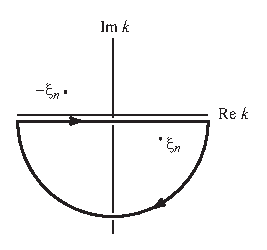
\includegraphics{../figures/chap11/fig02.eps}
\end{center}
\caption[Green contour]{\label{fig.Gcontour}
经过~$k\rightarrow -k$~这一替换,(\ref{eq:11.repre3})~式中的积分路径变为从~$-\infty-i0$~到 ~$\infty-i0$。
被积函数有两个面波极点,分别位于第四和第二象限。
在~$\Im{\rm m}\,k<0$~处闭合的积分环路包含~$\xi_n(\omega)$,但不包含~$-\xi_n(\omega)$。}
\end{figure}
\index{antipode}%
尽管如此,对所有奇偶数项行波震相的无穷求和在地球内部任何地方~$\bx$~都是确定的;
这当然是因为上式等价于驻波叠加~(\ref{eq:11.form})--(\ref{11.form2})。
我们将在下一节使用~(\ref{eq:11.repre3})~这个一致成立的结果来推导面波格林函数张量。
而在第~\ref{12.sec.Green}节中才会进一步考虑体波的响应。
\index{travelling wave|)}%

%\section{Surface-Wave Green Tensor}
\section{面波格林函数张量}
\index{tensor!Green!surface-wave|(}%
\index{Green tensor!surface-wave|(}%
\index{surface-wave Green tensor|(}%

在球对称地球上,任一基阶和高阶的勒夫和瑞利面波都是相互独立传播的。
要得到每条频散分支所对应的格林函数张量,对于固定的径向阶数~$n$~和震相序号~$s$,我们直接应用留数定理来计算~(\ref{eq:11.repre3})~式中对波数的积分。
对于一给定的角频率~$\om$,$\bG_n(k)$~在复数波数平面上有两个简单极点~$k=\pm\xi_n(\om)$。 从实际出发,我们在下文中假设~$\om>0$。
这样,极点均来自~(\ref{11.form2})~式中正频率的洛伦兹谱峰,并且由如下隐式确定
\eq \label{11.pole1}
\gamma_n(\xi_n)+i[\om-\om_n(\xi_n)]=0.
\en
在弱衰减极限下,将本征频率和衰减率在点~$k=k_n(\om)$~附近展开,
我们可以得到~$\xi_n(\om)$~的显式公式:
\eqa \label{11.pole2} \lefteqn{
\omn(\xi_n)=\om_n(k_n)+C_n(\xi_n-k_n)+\cdots} \nonumber \\
&&\mbox{}\hspace{3.3 mm}=\om+C_n(\xi_n-k_n)+\cdots,
\ena
\eq \label{11.pole3}
\gamma_n(\xi_n)\hspace{0.3 mm}=\gamma_n(k_n)+\cdots,
\en
其中~$k=k_n(\om)$~是扰动前弹性地球上频率为~$\om$~的波的实数波数,
省略号表示被忽略的高阶项。
为简单起见,也为了关注地震学所最感兴趣的问题,
我们将假设角本征频率~$\om_n$~沿每条频散分支是波数~$k>0$~的{\em 单调上升的\/}函数。
第~$n$~条频散曲线的正斜率
\eq \label{11.posCdefn}
C_n(\om)=\left(\frac{d\omn}{dk}\right)_{k=k_n(\omega),}
\en
则是对应的面波在单位球面上以弧度/秒为单位的角{\em 群速度\/}。
\index{group speed}%
\index{speed!group}%
将近似式~(\ref{11.pole2})--(\ref{11.pole3})~代入~(\ref{11.pole1}),
我们得到精确到一阶非弹性的极点表达式
\eq
\xi_n=k_n-i\gamma_n/C_n
=k_n-i\om/2C_nQ_n,
\label{eq:11.pole}
\en
其中~$Q_n(\om)$~是时间品质因子。
\index{temporal quality factor}%
\index{quality factor!temporal}%
\index{Q@{\em Q}!temporal}%
$C_n>0$~和~$Q_n>0$~的条件确保了面波极点~$\xi_n(\om)$~和~$-\xi_n(\om)$~分别位 于实轴的下方和上方一点,也就是在波数平面的第四和第二象限。

行波勒让德函数在~$k\rightarrow\infty$~极限时的渐进行为以及指数项~$\exp[-i(s-1)k\pi]$~和 ~$\exp(-isk\pi)$~的存在,要求我们在下半~$k$~平面闭合积分环路,以避免在使用留数定理计算~(\ref{eq:11.repre3})~中的积分时来自无穷远处的弧线部分的贡献。
因此,我们唯一环绕的极点是在第四象限的~(\ref{eq:11.pole}),如图~\ref{fig.Gcontour}所示。 通过计算留数,我们得到面波格林函数张量$\bG=\bG_{\rm Love}+\bG_{\rm Rayleigh}$
\eqa
\lefteqn{\bG=\half\sum_{n=0}^{\infty}(c_nC_n)^{-1}\biggl\{
\sum_{s=1,3,5,\ldots}^\infty\exp i[(s-2)\pi/2-(s-1)
\xi_n\pi]} \label{eq:11.travel} \nonumber \\
&&\mbox{}\qquad\qquad\times\bD_n\bD_n^{\prime}
Q_{\xi_n-\subhalf}^{(1)}(\cos\Theta) \nonumber \\
&&\mbox{}+\sum_{s=2,4,6,\ldots}^\infty
\exp i[(s-1)\pi/2-s\xi_n\pi] \nonumber \\
&&\mbox{}\qquad\qquad\times\bD_n
\bD_n^{\prime}Q_{\xi_n-\subhalf}^{(2)}(\cos\Theta)\biggr\}.
\ena
$c_n$~是面波的角{\em 相速度\/},
\index{phase speed}%
\index{speed!phase}%
\eq
c_n(\om)=\om/k_n(\om),
\en
而此时微分算子~$\bD_n=U_n\brh
+k_n^{-1}V_n\bdel_{\!1}-k_n^{-1}W_n
(\brh\times\bdel_{\!1})$~和~$\bD_n^{\prime}
=U_n^{\prime}\brh^{\raise-.2ex\hbox{$\scriptstyle\prime$}}+
\sqL_n^{-1}V_n^{\prime}\bdel_{\!1}^{\raise-.1ex\hbox{$\scriptstyle\prime$}}
-\sqL_n^{-1}W_n^{\prime}(\brh^{\raise-.2ex\hbox{$\scriptstyle\prime$}}
\times\bdel_{\!1}^{\raise-.1ex\hbox{$\scriptstyle\prime$}})$
~被视为是频率的函数。
(\ref{eq:11.travel})~这一表达式在完全弹性地球上是{\em 精确的\/},
而在非弹性地球上,则是精确到面波品质因子倒数~$Q_n^{-1}$~的一阶。
每一项表示一个从源点~$\Theta=0$~出发呈指数衰减的波;
与第二象限极点~$-\xi_n(\om)$~对应的呈指数增长的波被排除了。
奇数序号~$s=1,3,5,\ldots$~的震相对应于
\index{orbit}%
\index{surface-wave orbit}%
多周的勒夫和瑞利波群
${\rm G}1,\,{\rm G}3,\,{\rm G}5,\ldots$ 和
${\rm R}1,\,{\rm R}3,\,{\rm R}5,\ldots$,
偶数序号~$s=2,4,6,\ldots$~的震相则对应于
${\rm G}2,\,{\rm G}4,\,{\rm G}6,\ldots$ 和
${\rm R}2,\,{\rm R}4,\,{\rm R}6,\ldots$。

\begin{figure}
\begin{center}
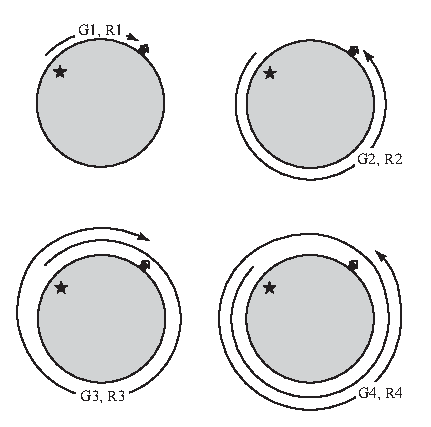
\includegraphics{../figures/chap11/fig03.eps}
\end{center}
\caption[G&Rorbits]{\label{11.fig.orbits}
多周面波的命名规则。
源点和地震台站分别以星号和狗舍表示。
字母~G~和~R~分别代表勒夫和瑞利面波;数字则表示到达接收点的序号。}
\end{figure}

在离开震中~$\Theta=0$~及其对跖点~$\Theta=\pi$~的地方,
当实数波数很大~$k_n\gg 1$,且非弹性较弱~$Q_n\gg 1$~时,
我们可利用行波勒让德函数的渐进近似:
\eqa \label{11.Qasy} \lefteqn{
Q_{\xi_n-\subhalf}^{(1,2)}(\cos\Theta)\approx
(2\pi k_n\sin\Theta)^{-1/2}} \nonumber \\
&&\mbox{}\times
\exp[\mp i(k_n\Theta-\pi/4)\mp\om\Theta/2C_nQ_n],
\ena
来简化~$\bG(\bx,\bx';\om)$。
由此得到的{\em 远场格林函数张量\/}可以写成对{\em 模式\/}或频散分支~$n=0,1,2,\ldots$
\index{tensor!Green!far-field}
\index{Green tensor!far-field}
\index{orbit}%
\index{surface-wave orbit}%
~和{\em 面波周数\/}或震相序号~$s=1,2,3,\ldots$~的双重求和
\eqa \label{11.dubsum} \lefteqn{
\bG(\bx,\bx';\om)=\sum_{\rm modes}\,\sum_{\rm rays}\hspace{1.0 mm}
(c\hspace{0.3 mm}C)^{-1}(8\pi k|\sin\Delta|)^{-1/2}} \\
&&\mbox{}\times[\brh U-i\bkh V+i(\brh\times\bkh)W]
[\brh' U'+i\bkh^{\raise-.65ex\hbox{$\scriptstyle\prime$}}
V'-i(\brh'\times\bkh^{\raise-.65ex\hbox{$\scriptstyle\prime$}})W']  \nonumber \\
&&\mbox{}\qquad\times\exp i\left[-k\Delta+(s-1)
\pi/2-\pi/4\right]\exp(-\om\Delta/2CQ), \nonumber
\ena
这里为简单起见我们略去了数字序号和角标。
给定震相所走过的总的角距离~$\Delta$~可由下面的显式给定
\eq
\Delta=\left\{\begin{array}{ll}
\Theta+(s-1)\pi, & \hspace{4.0 mm}\mbox{$s$ 为奇数} \\
\vspace{-1.0 mm} & \vspace{-1.0 mm} \\
s\pi-\Theta, & \hspace{4.0 mm}\mbox{$s$ 为偶数}.
\end{array}\right.
\en
对于~G1~和~R1~波,$\Delta=\Theta$;
对于~G2~和~R2~波, $\Delta=2\pi-\Theta$;
对于~G3~和~R3~波, $\Delta=\Theta+2\pi$;以此类推。
$\bkh$~和
~$\bkh^{\raise-.65ex\hbox{$\scriptstyle\prime$}}$
~是{\em 单位波矢量\/},
分别表示在~$\bx$~处的传播方向和在~$\bxh$~处的射线出射方向,即
\eq \label{11.kvecs}
\bkh=\left\{\begin{array}{rl}
\bThetah, & \mbox{$s$ 为奇数} \\
\vspace{-1.5 mm} & \vspace{-1.5 mm} \\
-\bThetah, & \mbox{$s$ 为偶数},
\end{array}\right. \quad\quad
\bkh^{\raise-.65ex\hbox{$\scriptstyle\prime$}}=\left\{\begin{array}{rl}
\bThetahpr, & \mbox{$s$ 为奇数} \\
\vspace{-1.5 mm} & \vspace{-1.5 mm} \\
-\bThetahpr, & \mbox{$s$ 为偶数},
\end{array}\right.
\en
\eq \label{11.rkvecs}
\brh\times\bkh=\left\{\begin{array}{rl}
\bPhih, & \mbox{$s$ 为奇数} \\
\vspace{-1.5 mm} & \vspace{-1.5 mm} \\
-\bPhih, & \mbox{$s$ 为偶数},
\end{array}\right. \quad\quad
\brh'\times\bkh^{\raise-.65ex\hbox{$\scriptstyle\prime$}}
=\left\{\begin{array}{rl}
\bPhihpr, & \mbox{$s$ 为奇数} \\
\vspace{-1.5 mm} & \vspace{-1.5 mm} \\
-\bPhihpr, & \mbox{$s$ 为偶数}.
\end{array}\right.
\en
从物理上讲,我们可以把~$\brh$、$\bkh$~和~$\brh\times\bkh$
~当作以顺时针或逆时针方向绕地球传播的面波的径向、纵向和横向偏振方向,
\index{surface-wave polarization}%
\index{polarization!surface-wave}%
如图~\ref{11.fig.rkvecs}所示。
值得注意的是,当~$\bx$~和~$\bx'$~互换时,传播方向也反转了,即
~$\bkh\rightarrow -\bkh$~和~$\bkh^{\raise-.65ex\hbox{$\scriptstyle\prime$}}
\rightarrow -\bkh^{\raise-.65ex\hbox{$\scriptstyle\prime$}}$,因此
远场格林函数张量~(\ref{11.dubsum})~满足源点-接收点互易性原理~$\bG(\bx,\bx';\om)=\bG^{\rm T}(\bx',\bx;\om)$。
\index{reciprocity!surface waves}%

如前所述,本节的结果仅适用于正的角频率,即~$\om>0$。
$\om<0$~的结果可以简单地将留数定理应用到与负频率的洛伦兹谱峰~$\gamma_n(\xi_n)+i[\om+\om_n(\xi_n)]=0$~对应的第三象限面波极点而得到。
或者利用时间域响应~$\bG(\bx,\bx';t)$~为实数这一规律所带来的普遍关系式~$\bG(\bx,\bx';-\om)=\bG^*(\bx,\bx';\om)$,我们也可以更简单地得到这一结果。
$\bG(\bx,\bx';\om)$~中所依赖的是~$\exp(-ik\Delta)$~而非
~$\exp(ik\Delta)$,这需要回溯到在~(\ref{4.FTdef})~和~(\ref{11.FTG})~的傅里叶变换中我们所选用的符号习惯。
从震源向外传播的波的表达式是~$\exp\hspace{0.1 mm}i(\om t-k\Delta)$~而非
~$\exp\hspace{0.1 mm}i(k\Delta-\om t)$。
\begin{figure}[!t]
\begin{center}
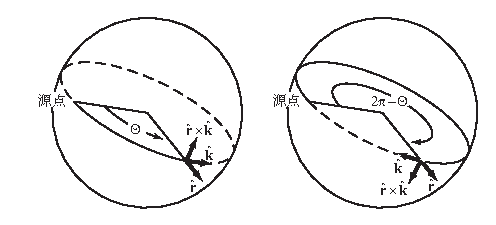
\includegraphics{../figures/chap11/fig04.eps}
\end{center}
\caption[r&kvectors]{\label{11.fig.rkvecs}
面波射线路径示意图,G1~或~R1~面波走过长度为~$\Theta$~的劣弧~({\em 左图\/}),而~G2~或~R2~面波则走过长度为~$2\pi-\Theta$~的优弧~({\em 右图\/})。
粗箭头表示接收点处的径向、纵向和横向单位偏振矢量~$\hat{\bf r}$, $\hat{\bf k}$~和~$\hat{\bf r}\times\hat{\bf k}$。
}
\end{figure}

在某些极不寻常的场合,
自引力地球上基阶和高阶模式的瑞利波的
\index{self-gravitation!effect on wavenumber}%
本征频率~$\om_n$~可能是随波数~$k>0$~{\em 递减\/}而非递增的函数~(Gilbert \citeyear{gilbert67})。
在这种情况下,角群速度的定义是~$C_n=-(d\om/dk)_{k=k_n}$~而不是~(\ref{11.posCdefn}),
而且面波极点~$\xi_n$~和~$-\xi_n$~分别位于第三和第一象限,而非第四和第二象限。
当积分环路在下半~$k$~平面闭合时,只有第三象限的极点有贡献;
由此得到的远场格林函数张量与~(\ref{11.dubsum})~完全相同,
只是相位因子~$\exp(-ik\Delta)$~被~$\exp(ik\Delta)$~取代。
从而每个单频波的形式都是~$\exp\hspace{0.1 mm}i(\om t+k\Delta)$;也就是说,单独的波峰和波谷都是向着源点传播的,而不是离开源点。
但不论频散的特性如何,群速度固有的正值性~$C_n>0$~保证了
相关的波动能量总是从宽频的地震震源向外传播的。
在本书的剩余部分中,我们将继续着眼于具有~$d\om/dk>0$~的“正常”频散的波动。
\index{tensor!Green!surface-wave|)}%
\index{Green tensor!surface-wave|)}%
\index{surface-wave Green tensor|)}%

%\section{Moment-Tensor Response}
\section{矩张量响应}
\index{moment-tensor response!surface waves|(}%
\index{response!surface-wave|(}%
\index{surface-wave response|(}%
\label{sec.11.resp}

一个阶跃函数、矩张量源的加速度响应的驻波表达式为
\eqa \lefteqn{
\ba=\frac{1}{2\pi}\sum_{n=0}^{\infty}\sum_{l=0}^{\infty}
(l+\half)\left[\frac{\half}{\gammanl+i(\om-{}_n\om_l)}
+\frac{\half}{\gammanl+i(\om+{}_n\om_l)}\right]} \nonumber \\
&&\mbox{}\times{}_n\bD_l\sum_{m=0}^2P_{lm}(\cos\Theta)
(A_m\cos m\Phi+B_m\sin m\Phi),
\ena
这里为更大的适用性起见,我们保留了~(\ref{10.accfreq})--(\ref{10.Lorentz})~中被丢掉的负频率洛伦兹谱峰。
相应的行波表达式可以通过直接推广前面的推导,即
使用泊松叠加公式~(\ref{eq:11.Poisson}),
将相关的勒让德函数分解成以下形式
\eq
P_{k-\subhalf\,m}(\cos\Theta)=Q_{k-\subhalf\,m}^{(1)}(\cos\Theta)
+Q_{k-\subhalf\,m}^{(2)}(\cos\Theta),
\en
并改变积分环路的形状,使其成为在实数波数轴下面一点从~$-\infty-i0$到$\infty-i0$。
由此得到表达式
\eqa \label{eq:11.acctrave}
\lefteqn{\ba=\frac{1}{2\pi}\sum_{n=0}^{\infty}
\biggl\{\sum_{s=1,3,5,\ldots}^\infty(-1)^{(s-1)/2}
\int_{-\infty}^\infty\an(k)
\,\bD_n\sum_{m=0}^2Q_{k-\subhalf\,m}^{(1)}(\cos\Theta)} \nonumber \\
&&\mbox{}\qquad\times(A_m\cos m\Phi+B_m\sin m\Phi)
\,e^{-i(s-1)k\pi}\,kdk \nonumber \\
&&\mbox{}+\sum_{s=2,4,6,\ldots}^\infty
(-1)^{s/2}\int_{-\infty}^\infty\an(k)
\,\bD_n\sum_{m=0}^2Q_{k-\subhalf\,m}^{(2)}(\cos\Theta) \nonumber \\
&&\mbox{}\qquad\times(A_m\cos m\Phi+B_m\sin m\Phi)
\,e^{-isk\pi}\,kdk\biggr\},
\ena
其中我们引入了变量
\eq
\an(k)=\frac{\half}{\gamma_n(k)+i[\om-\omn(k)]}
+\frac{\half}{\gamma_n(k)+i[\om+\omn(k)]}.
\label{eq:11.ank}
\en
如同~(\ref{eq:11.repre3})~式,上述结果同时适用于体波和面波;
如果把实数算子~$\bD_n$~用复数的~$\bsD_n$~替换,
并把实的系数~$A_m$~and~$B_m$~也用复的~$\sA_m$~和~$\sB_m$~替换,
该式甚至在非弹性地球上也是精确的。

要得到面波响应~$\ba=\ba_{\rm Love}+\ba_{\rm Rayleigh}$,
对于每一个固定的频散分支~$n$~和每一个奇偶序号~$s$~的波群震相,
我们应用留数方法来计算~(\ref{eq:11.acctrave})~中对波数的积分。
由此得到类似于~(\ref{eq:11.travel})~的表达式
\eqa
\lefteqn{\ba=\half i\om\sum_{n=0}^{\infty}(c_nC_n)^{-1}\biggl\{
\sum_{s=1,3,5,\ldots}^\infty\exp i[(s-2)\pi/2-(s-1)
\xi_n\pi]} \label{11.accresp} \nonumber \\
&&\mbox{}\times\bD_n
\sum_{m=0}^2Q_{\xi_n-\subhalf\,m}^{(1)}(\cos\Theta)
(A_m\cos m\Phi+B_m\sin m\Phi) \nonumber \\
&&\mbox{}+\sum_{s=2,4,6,\ldots}^\infty
\exp i[(s-1)\pi/2-s\xi_n\pi] \\
&&\mbox{}\times\bD_n
\sum_{m=0}^2Q_{\xi_n-\subhalf\,m}^{(2)}(\cos\Theta)
(A_m\cos m\Phi+B_m\sin m\Phi)\biggr\}. \nonumber
\ena
(\ref{11.accresp})~式在地球内部的任何地方都一致成立;
在离开震中及其对跖点的地方,我们可以利用渐近表达式~(\ref{11.Qasy})~的~$0\leq m\leq 2$~的广义形式来进行化简:
\eqa \label{11.Qmasy} \lefteqn{
Q_{\xi_n-\subhalf\,m}^{(1,2)}(\cos\Theta)\approx(-k_n)^m
(2\pi k_n\sin\Theta)^{-1/2}} \nonumber \\
&&\mbox{}\times
\exp[\mp i(k_n\Theta+m\pi/2-\pi/4)
\mp\om\Theta/2C_nQ_n].
\ena
类似于远场格林函数张量~(\ref{11.dubsum}),
用这种方式得到的地震的远场响应也可以写为对面波模式和射线的双重求和:
\eqa \label{11.accsum} \lefteqn{
\ba(\bx,\om)=\sum_{\rm 模式}\,\sum_{\rm 射线}\hspace{1.0 mm}
(c\hspace{0.3 mm}C)^{-1}(8\pi k|\sin\Delta|)^{-1/2}
[\brh U-i\bkh V+i(\brh\times\bkh)W]} \nonumber \\
&&\mbox{}\qquad\times R(\Phi)\exp i\left[-k\Delta+(s-1)
\pi/2\right]\exp(-\om\Delta/2CQ),
\ena
其中
\eqa \label{11.radpat} \lefteqn{
R(\Phi)=\om\big\{[M_{rr}\dot{U}_{\rm s}+(M_{\theta\theta}+M_{\phi\phi})
r_{\rm s}^{-1}(U_{\rm s}-\half kV_{\rm s})]e^{i\pi/4}} \nonumber \\
&&\mbox{}+(-1)^s(\dot{V}_{\rm s}-r_{\rm s}^{-1}V_{\rm s}
+kr_{\rm s}^{-1}U_{\rm s})
(M_{r\phi}\sin\Phi+M_{r\theta}\cos\Phi)e^{-i\pi/4} \nonumber \\
&&\mbox{}-kr_{\rm s}^{-1}V_{\rm s}[M_{\theta\phi}\sin 2\Phi+\half(
M_{\theta\theta}-M_{\phi\phi})\cos 2\Phi]e^{i\pi/4} \nonumber \\
&&\mbox{}+(-1)^s(\dot{W}_{\rm s}-r_{\rm s}^{-1}W_{\rm s})
(M_{r\theta}\sin\Phi-M_{r\phi}\cos\Phi)e^{-i\pi/4} \nonumber \\
&&\mbox{}-kr_{\rm s}^{-1}W_{\rm s}[\half(M_{\theta\theta}
-M_{\phi\phi})\sin 2\Phi-M_{\theta\phi}\cos 2\Phi]e^{i\pi/4}\big\}.
\ena
(\ref{11.radpat})~式中~$U_{\rm s}$、$V_{\rm s}$~和~$W_{\rm s}$~的罗马字母下角标表示在震源的半径~$r_{\rm s}$~处取值;
它们不应与斜体的波群震相角标~$s$~混淆。
普遍结果~(\ref{11.accresp})~和远场结果~(\ref{11.accsum})~都仅适用于正频率~$\om>0$;
负频率~$\om<0$~的表达式可以借由对称性~$\ba(\bx,-\om)=\ba^*(\bx,\om)$~而得到。

表达式~(\ref{11.accsum})中的每一项都有直接的物理意义。
振荡因子$\exp(-ik\Delta)=\exp(-i\om\Delta/c)$ 表示沿着大圆面波射线路径以角速度$c$传播过角距离$\Delta$的相位延迟。
矢量$\brh U-i\bkh V+i(\brh\times\bkh)W$描述面波到达接收点时的{\em 偏振\/};
\index{polarization!surface-wave}%
\index{surface-wave polarization}%
在长波长$k\gg 1$极限下,
勒夫波表现为纯粹的横向质点运动$i(\brh\times\bkh)W$,
\index{particle motion!Love-wave}%
\index{polarization!Love-wave}%
\index{Love-wave polarization}%
而瑞利波则表现出径向和纵向运动。
瑞利波偏振$\brh U-i\bkh V$中的因子$i$暗示了质点运动是椭圆形的,
\index{particle motion!Rayleigh-wave}%
\index{polarization!Rayleigh-wave}%
\index{Rayleigh-wave polarization}%
即在${\rm sgn}\,U\not={\rm sgn}\,V$的深度为逆进椭圆,
而在${\rm sgn}\,U={\rm sgn}\,V$的深度则为顺进椭圆。
振幅因子$|\sin\Delta|^{-1/2}$来自球面上单频面波的{\em 几何扩散\/}。
\index{geometrical spreading!surface waves}%
在球面上,
一个无穷窄的面波射线束的微分角宽度与震中距正弦的绝对值成正比:$dw\propto|\sin\Delta|$。
如果不考虑非弹性耗散,射线束中的波动能量是守恒的;
因而与波动能量的平方根成正比的波的振幅$A$的变化形式为
\eq
\frac{A_2}{A_1}=\left(\frac{dw_2}{dw_1}\right)^{-1/2}=
\left|\frac{\sin\Delta_2}{\sin\Delta_1}\right|^{-1/2},
\en
其中下角标1和2分别表示射线束上的前后两点。
指数衰减因子$\exp(-\om\Delta/2CQ)$来源于地球内部因摩擦力的存在而造成的面波额外的{\em 非弹性衰减\/};
\index{attenuation!surface-wave}%
\index{surface-wave attenuation}%
分母中的因子是$C$而不是$c$,这反应了被耗散的波动能量是以群速度传播的。
因子$\exp[i(s-1)\pi/2]$是所谓的"球极"相移,
\index{phase shift!polar}%
\index{polar phase shift}%
其重要性也是由Brune, Nafe \& Alsop (\citeyear{brune&al61})首次在这样的意义下指出的。
而事实上,这种每次在通过对跖点和源点时所发生的与频率无关的$\pi/2$相位提前
是{\em 焦散相移\/}这一更为普遍现象的一个特例。
\index{caustic phase shift}%
\index{phase shift!caustic}%
如果将射线束的微分宽度视为一个随着总的传播距离而平滑变化的正负值函数,
即$dw\propto\sin\Delta$,
那么我们便可以将这一相移与伴随着每次通过焦散时的符号变化${\rm sgn}\hspace{0.7 mm}dw_2\not={\rm sgn}\hspace{0.7 mm}dw_1$关联起来:
\eq \label{11.piover2}
\left(\frac{dw_2}{dw_1}\right)^{-1/2}=
\left(\frac{\sin\Delta_2}{\sin\Delta_1}\right)^{-1/2}
=\left|\frac{\sin\Delta_2}{\sin\Delta_1}\right|^{-1/2}\exp(i\pi/2).
\en
最后,(\ref{11.radpat})式所给定的依赖频率的$R(\Phi)$代表的是
复数的{\em 勒夫或瑞利波辐射花样\/}。
\index{radiation pattern!surface-wave}%
\index{surface-wave radiation pattern}%
\index{Love-wave radiation pattern}%
\index{Rayleigh-wave radiation pattern}%
对于一已知震源位置$\bx_{\rm s}$和矩张量$\bM$,
(\ref{11.accsum}) 和~(\ref{11.radpat})两式提供了测量和解释面波相速度$c$和品质因子$Q$的一个依据。
反之,如果将相速度$c$和品质因子$Q$视为已知,我们可以利用上述结果
用${\rm G}1,\,{\rm G}2, \,{\rm G}3,\ldots$
或${\rm R}1,\,{\rm R}2,\,{\rm R}3,\ldots$面波的频谱来确定地震的深度和震源机制$\bM$。
除了对很长周期的面波外,自由空气、倾斜和势函数微扰对所有面波的影响都很小;
然而,这些影响是很容易考虑的,
只需简单地将~(\ref{11.accsum})中的偏振矢量以其做引力修改后的形式替换即可:
$\brh U-i\bkh V+i(\brh\times\bkh)W\rightarrow
\brh U_{\hspace{-0.2 mm}\star}-i\bkh V_{\hspace{-0.3 mm}\star}
+i(\brh\times\bkh)W$。

%The result~(\ref{11.accsum})--(\ref{11.radpat}) can alternatively
%be obtained by starting with the far-field surface-wave Green
%tensor~(\ref{11.dubsum}) and applying the general formula
(\ref{11.accsum})--(\ref{11.radpat})两式的另一种推导也可以
从远场格林函数张量~(\ref{11.dubsum})出发,并使用下面的普遍表达式
\eq \label{11.aeqMdotG}
\ba(\bx,\om)=i\om\hspace{0.2 mm}\bM\!:\!\bdel_{\!\rm s}
\bG^{\rm T}(\bx,\bx_{\rm s};\om).
\en
在最低阶近似下,相对于震源坐标$\bx_{\rm s}$的梯度$\bdel_{\!{\rm s}}=
\brh_{\rm s}\p_{r_s}+r_{\rm s}^{-1}\bdel_{\!1{\rm s}}$
仅作用于振荡项$\exp(-ik\Delta)$和震源偏振矢量$\brh_{\rm s}U_{\rm s}
+i\bkh_{\rm s}V_{\rm s}-i(\brh_{\rm s}\times
\bkh_{\rm s})W_{\rm s}$上。
辐射花样~(\ref{11.radpat})可以用不变量符号改写成以下形式
\eq \label{11.radpat2}
R(\Phi)=i\om(\bM\!:\!\bE_{\rm s}^*)\exp(-i\pi/4).
\en
复对称张量
\eqa
\lefteqn{\bE_{\rm s}=\dU_{\!\rm s}\brh_{\rm s}\brh_{\rm s}
+r_{\rm s}^{-1}(U_{\rm s}-kV_{\rm s})\bkh_{\rm s}\bkh_{\rm s}
+r_{\rm s}^{-1}U_{\rm s}(\brh_{\rm s}\times\bkh_{\rm s})
(\brh_{\rm s}\times\bkh_{\rm s})} \nonumber \\
&&-\half i(\dV_{\rm s}-r_{\rm s}^{-1}V_{\rm s}
+kr_{\rm s}^{-1}U_{\rm s})(\brh_{\rm s}\bkh_{\rm s}
+\bkh_{\rm s}\brh_{\rm s}) \nonumber \\
&&\mbox{}\quad+\half i(\dW_{\!\rm s}-r_{\rm s}
^{-1}W_{\rm s})[\brh_{\rm s}(\brh_{\rm s}\times\bkh_{\rm s})
+(\brh_{\rm s}\times\bkh_{\rm s})\brh_{\rm s}] \nonumber \\
&&\quad\qquad+\half kr_{\rm s}^{-1}W_{\rm s}
[\bkh_{\rm s}(\brh_{\rm s}\times\bkh_{\rm s})
+(\brh_{\rm s}\times\bkh_{\rm s})\bkh_{\rm s}] \label{11.strain}
\ena
是震源处的{\em 面波应变\/}。
\index{strain!surface-wave}%
\index{surface-wave strain}%
在第~16.5节中,我们会用JWKB近似将远场脉冲和矩张量响应~(\ref{11.dubsum})和~(\ref{11.accsum})--(\ref{11.radpat})推广到光滑的横向不均匀地球模型。
和~(\ref{11.accsum})--(\ref{11.radpat})。
\index{moment-tensor response!surface waves|)}%
\index{response!surface-wave|)}%
\index{surface-wave response|)}%

%\section{Stationary-Phase Approximation}
\section{稳相近似}
\index{stationary-phase approximation|(}%
\label{11.sec.group}

勒夫和瑞利波传播的一个显着特征是相速度$c=\om\hspace{-0.2 mm}/\hspace{-0.2 mm}k$依赖于波数$k$和频率$\om$。
由于不同波数和频率的波以不同的速度传播,
从位置固定的震源所发出的讯号在不同的时间到达,因此这样的传播被称为是{\em 频散的\/}。
\index{dispersion!surface-wave}%
\index{surface-wave dispersion}%
在本节中,我们将回顾众所周知的群速度~$C=d\om\hspace{-0.3 mm}/\hspace{-0.3 mm}dk$在运动学和能量上的重要意涵。
如果我们视相速度$c$为波数$k$的函数,则群速度和相速度的关系为
\index{phase speed}%
\index{group speed}%
\index{speed!group}%
\index{speed!phase}%
\eq
C=d(ck)\hspace{-0.2 mm}/\hspace{-0.3 mm}dk=c+k(dc/\hspace{-0.3 mm}dk).
\en
另一方面,如果我们将$c$视为频率$\om$的函数,则有
\eq \label{11.Ccreln}
C=\frac{c}{1-(\om\hspace{-0.1 mm}/\hspace{-0.1 mm}c)
(dc/\hspace{-0.3 mm}d\omega)}.
\en
这里所呈现的结果都不是地震面波所特有的;
事实上,它们适用于任何线性介质中的频散波动。
\textcite{whitham74}和\textcite{lighthill78}中有对线性频散波动传播更系统和权威的论述。
在\textcite{bender&orszag78}中对作为相关分析的重要数学基础的{\em 稳相方法\/}有更严格的阐述。
\index{method of stationary phase}%

\iffalse
Every mode branch $n=0,1,2,\ldots$ and multi-orbit
arrival $s=1,2,3,\ldots$ in the response~(\ref{11.accsum})
is subjected to an independent kinematic analysis; the
double summation over modes and surface-wave rays
will henceforth be regarded as understood.
Each term in the sum may be written in the abbreviated form
\fi
在~(\ref{11.accsum})的响应中,对每一径向模式分支$n=0,1,2,\ldots$与每一多周震相$s=1,2,3,\ldots$ 可以进行独立的运动学分析;因此在后续分析中对模式和面波射线的双重求和将被视为是不言而喻的。叠加中的每项都可以用简化的形式表示为
\eq
\ba(\bx,\om)=\bA(\bx,\om)\exp[-ik(\om)\Delta],
\label{eq:11.bs}
\en
其中
\eqa
\lefteqn{\bA=\om(c\hspace{0.3 mm}C)^{-1}(8\pi k|\sin\Delta|)^{-1/2}
[\brh U-i\bkh V+i(\brh\times\bkh)W]} \nonumber \\
&&\mbox{}\times R(\Phi)\exp [i(s-1)
\pi/2]\exp(-\om\Delta/2CQ). \label{11.ampdef}
\ena
要注意的是,非弹性阻尼$\exp(-\om\Delta/2CQ)$和几何扩散$|\sin\Delta|^{-1/2}$
均已被包含在振幅因子$\bA(\bx,\om)$中。
当非弹性较弱时,这样做总是允许的;
在实际中,这两种效应所造成的振幅变化数量级相同。
单一模式、单一射线的时间域响应可通过计算~(\ref{eq:11.bs})的傅立叶反变换得到:
\eq \label{11.four}
\ba(\bx,t)=\frac{1}{\pi}\,\Re{\rm e}\!\int_{0}^\infty
\bA(\bx,\om)\exp[i\om t-ik(\omega)\Delta]\,d\om,
\en
这里我们使用了等式$\ba(\bx,-\om)=\ba^*(\bx,\om)$来计算上述单边积分。
通过定义
\eq
\Psi(\om)=\om-k(\om)\Delta/t,
\en
我们可以将~(\ref{11.four})改写为适于应用稳相方法的形式,
\eq
\ba=\frac{1}{\pi}\,\Re{\rm e}\!\int_{0}^\infty
\bA(\om)\exp[it\Psi(\om)]\,d\om,
\label{11.four2}
\en
其中不重要的自变量略去不写。
我们试图{\em 对固定的参数值\/} $\Delta/t$,在$t\rightarrow\infty$的极限下,
渐近地计算加速度~(\ref{11.four2});
由此得到的响应将是一个以固定速度移动中的观察者所看到的。
基本的思路是,被积函数在时间很长时是高度振荡的,因而导致高度的相互抵消,
只有在具稳定性的相位$\Psi(\om)$处频率相近的波得以彼此相互加强。

令$\om_0$为~(\ref{11.four2})中被积函数的相位稳定的角频率(或许不止一个频率):
\eq \label{11.CDt}
\Psi'(\om_0)=0.
\en
在本节剩余的部分,我们用撇号表示相对于频率的微分,
即$d/\hspace{-0.2 mm}d\om$,
用下标$0$表示在稳定角频率处的值,如$C_0=C(\om_0)$。
(\ref{11.CDt})式等价于以下结果
\eq \label{11.CDt2}
\Delta/t=C_0,
\en
因此上面提到的观察者是以稳定的群速度$C_0$在移动。
在$t\rightarrow\infty$的极限下,加速度$\ba$ 完全由紧邻稳相点$\om_0$附近的频率所决定。
在该邻近区域,我们可将~(\ref{11.four2})中的的振幅和相位分别用零阶和二阶泰勒展开来近似
\eq
\bA(\om)\approx\bA_0,\qquad\quad\Psi(\om)\approx\Psi_0
+\half(\om-\om_0)^2\Psi''_0.
\label{11.taylor}
\en
值得注意的是,由于$\Psi_0^{\prime}=0$,因而没有与$\om-\om_0$成正比的相位项。
利用~(\ref{11.taylor})中的近似,我们得到
\eqa \label{11.four3} \lefteqn{
\ba\approx\frac{1}{\pi}\,\Re{\rm e}\,\bigg\{\bA_0
\exp[i(\om_0t-k_0\Delta)]} \nonumber \\
&&\mbox{}\qquad\qquad\qquad\times\int_{-\infty}^{\infty}
\exp\left[\half i\Psi''_0(\om-\om_0)^2t\right]d\om\bigg\},
\ena
这里我们反过来利用同样的相互抵消的逻辑,
将积分限从(\ref{11.taylor})成立的$\om_0$附近的狭窄区间
扩展到整个频率轴$-\infty\leq\omega\leq\infty$。
将积分路径旋转$\pm\pi/4$,
~(\ref{11.four3})中保留的积分可以解析地计算出来:
\eqa
\lefteqn{\int_{-\infty}^{\infty}
\exp\left[\half i\Psi''_0(\om-\om_0)^2t\right]d\om} \nonumber \\
&&\qquad\qquad\qquad\mbox{}=\left(\frac{2\pi C_0}{|C'_0|t}\right)^{1/2}
\exp(\fourth i\pi\,{\rm sgn}\,C'_0),
\ena
这里我们用到了$\Psi''_0=C'_0/\hspace{-0.2 mm}C_0$这一事实。
因此,响应$\ba(\bx,t)$简化为
\eq
\ba\approx\Re{\rm e}\left[\bsA
\exp i\left(\om_0t-k_0\Delta
\right)\right],
\label{11.bsasmp}
\en
其中
\eq \label{11.bsasmp2}
\bsA=\bA_0\left(\frac{2C_0}
{\pi|C'_0|t}\right)^{1/2}
\exp(\fourth i\pi\,{\rm sgn}\,C'_0).
\en
$t\rightarrow\infty$这一条件确保波是在很久之前离开源点的,因而有充分的频散。
这样在角震中距$\Delta$处$t$时刻的渐近讯号看起来是由频率$\om_0$、
波数$k_0$和$\bsA$可变的{\em 单个波\/}所组成。
如果存在一个以上的稳相频率$\om_0$,
则上述响应是形如~(\ref{11.bsasmp})--(\ref{11.bsasmp2})的项的叠加。

稳定性条件~(\ref{11.CDt2})表明$\Delta=C_0t$是所有频率为$\om_0$、波数为$k_0$的波在$t$时刻所处的位置;
以速度$C_0$离开源点的观察者始终被该频率与波数的波{\em 群\/}所包围,这也正是名称的由来。
\index{wavegroup}%
组成波群的单独波始终在变化,因为它们是以相速度$c_0$传播的。
究竟新的波峰和波谷是从背后进入波群再从前面离开,还是相反,这都取决于$c_0>C_0$ 还是 $c_0<C_0$。
从~(\ref{11.Ccreln})式可以看出,如果$c'_0<0$则相速度大于群速度,
而如果$c'_0>0$则群速度大于相速度。
单独的波峰或波谷必定会随时间加速或减速,因为其频率$\om$、波数$k$ 和相速度 $c$都不断在变化。
在固定的震中距$\Delta$,(\ref{11.CDt2})这一条件确定了面波地震图在$t$时刻的瞬时频率$\om_0$;
另一方面,在固定的时刻$t$,它确定了波列“快照"在距离$\Delta$处的局地波数$k_0$。

绝对振幅$\sA=|\bsA|$依赖于沿射线上的时间和距离,这可以通过考虑一块无穷小波群的能量来理解,
波群在两边被射线束外壁、前后被与频率$\om_0$和$\om_0+d\om_0$相对应的两条波群线所包围。
沿射线上任意一点,该波群块的微分表面积为
$d\/\Sigma=|\sin\Delta|\,d\/\Delta\,d\/\Phi=C'_0\hspace{0.2 mm}t\,|\sin\Delta|\,d\om_0\,d\/\Phi$,
其中我们将$C(\om_0)=\Delta/t$与
$C(\om_0+d\om_0)=(\Delta+d\/\Delta)/t$联立得到第二个等式。
在不考虑非弹性衰减时,该小块内所含有的能量为一常数;
因此在完全弹性地球上,前后两点处的振幅之间有如下关系
\eq \label{11.ratio2}
\frac{\sA_2}{\sA_1}
=\left(\frac{d\Sigma_2}{d\Sigma_1}
\right)^{-1/2}=\left|\frac{t_2\sin\Delta_2}
{t_1\sin\Delta_1}\right|^{-1/2}.
\en
由于频散,小波群块的前、后波群线以与$t$成正比的速率分离;
因此,波群的振幅$\sA$以$t^{-1/2}$的形式减小。
呈$t^{-1/2}$的频散衰减是叠加在单频波的几何扩散$|\sin\Delta|^{-1/2}$和非弹性$\exp(-\om\Delta/2CQ)$的振幅变化之上的。 
弹性振幅比值~(\ref{11.ratio2})与~(\ref{11.bsasmp})--(\ref{11.bsasmp2})的一致性
证实了{\em 能量以群速度传播\/}。
上述论证仅建立在能量与振幅的平方成正比的前提下;
在第16章中我们对面波行波的能量做一个更精确的定义,
并将我们在此发展的理论拓展到横向不均匀地球模型。

当$C'_0=0$,即在群速度的极大值或极小值附近,与极值两侧稳定点相应的波发生干涉,
(\ref{11.bsasmp})--(\ref{11.bsasmp2})中的渐近结果不成立;
这一干涉会产生一种振幅特别高的面波讯号,被称为{\em 艾里震相\/},
\index{Airy phase}%
\index{phase!Airy}%
以纪念艾里在研究光在焦散处衍射的相关数学问题中的杰出工作。
先将相位$\Psi(\om)$展开到$(\om-\om_0)^3$阶,然后计算响应,便可以得到一个包含了干涉主要特征的解析表达式(Ben-Menahem \& Singh \citeyear{ben-menahem&singh81});  然而,这种高阶的结果没有什么实际用途。
在定量的应用中,最好彻底放弃稳相近似,
而直接在频率域中采用表达式~(\ref{eq:11.bs})--(\ref{11.ampdef}),
或者数值计算傅里叶反变换~(\ref{11.four})。
此外,也可以通过叠加等价的简正模式${}_n{\rm T}_l$和${}_n{\rm S}_l$来计算面波响应$\ba(\bx,t)$。
(\ref{11.bsasmp})--(\ref{11.bsasmp2})中的近似结果的价值在于它为频散波传特性给予深刻的物理解释。
\index{stationary-phase approximation|)}%

%\section{Dispersion Relation and Group Speed}
\section{频散关系和群速度}
\index{dispersion relation|(}%
\index{group speed|(}%
\index{speed!group|(}%
\label{11.sec.disper}

任何以行波的波数$k$来表示其角频率$\om$的方程,都叫做{\em 频散关系\/}。
\index{dispersion relation}%
每一个基阶($n=0$)或高阶勒夫或瑞利面波分支的独立传播都受到各自频散关系的控制。
依照\textcite{jeffreys61},我们引入一个新的便利符号来描述球对称地球上面波的频散,
将它与瑞利原理一起用来推导一个有用的群速度$C=d\om/dk$表达式。
本节中的大部分内容只是简单地将第8章中所得到的结果用连续的波数$0\leq k\leq\infty$而非离散的球谐函数次数$l=0,1,2,\ldots$做重新的表述。

%\subsection{Love waves}
\subsection{勒夫波}
\index{Love wave|(}%
\index{surface wave!Love|(}%
\label{11.sec.LoveC}

控制勒夫波传播的作用量的径向积分~(\ref{8.spheractor})可以改写为
\eq \label{11.torI}
\sI=\half(\om^2I_1-k^2I_2-I_3),
\en
其中
\eq \label{11.Lint1}
I_1=\int_0^a\rho W^2\,r^2dr,
\en
\eq \label{11.Lint2}
I_2=\int_0^a\mu W^2\,dr,
\en
\eq \label{11.Lint3}
I_3=\int_0^a\mu[(\dW-r^{-1}W)^2-2r^{-2}W^2]\,r^2dr.
\en
在实际中,可以将(\ref{11.Lint1})--(\ref{11.Lint3})中的积分局限在地幔中$b\le r\le s$,
因为我们对于在固态内核中传播的面波并不感兴趣。
我们可以将能量均分关系$\sI=0$视为勒夫波的频散关系:
\index{Love-wave dispersion}%
\index{dispersion!Love-wave}%
\eq
\om^2I_1-k^2I_2-I_3=0.
\label{11.tordisp}
\en
方程~(\ref{11.tordisp})是频率$\om$与波数$k$的隐式关系式,
因为径向本征函数$W$是依赖于这些变量的。
勒夫波的动能加势能~(\ref{8.TOTOREN})也可以用~(\ref{11.Lint1})--(\ref{11.Lint3})中的积分来表示:
\index{energy!Love-wave}%
\index{Love-wave energy}%
\eq \label{11.Lovenergy}
\sE=\half(\om^2I_1+k^2I_2+I_3).
\en

瑞利原理要求,当且仅当$W$是角频率为$\om$、波数为$k$的勒夫波的本征函数时,
作用量~(\ref{11.torI})相对于微扰$W\rightarrow W+\delta W$是稳定的:
\eq
\om^2\delta\hspace{-0.2 mm}I_1-k^2\delta\hspace{-0.2 mm}I_2
-\delta\hspace{-0.2 mm}I_3=0,
\label{11.pertor}
\en
其中
\eq
\delta\hspace{-0.2 mm}I_1=2\int_0^a\rho W\,\delta W\,r^2dr,
\en
\eq
\delta\hspace{-0.2 mm}I_2=2\int_0^a\mu W\,\delta W\,dr,
\en
\eqa \lefteqn{
\delta\hspace{-0.3 mm}I_3=2\int_0^a\mu [(\dW-r^{-1}W)
(\delta\dW-r^{-1}\delta W)} \nonumber \\
&&\mbox{}\qquad\qquad\qquad-2r^{-2}W\,\delta W ]\,r^2dr.
\ena
另一方面,将频率为$\om$和$\om+\delta\om$、
波数为$k$和$k+\delta\hspace{-0.1 mm}k$以及径向本征函数为$W$和$W+\delta W$
的两个波的频散关系相减,我们得到
\eq
2\om\,\delta\om\,I_1 + \om^2\delta\hspace{-0.2 mm}I_1
-2k\,\delta\hspace{-0.1 mm}k\,I_2-k^2\delta\hspace{-0.2 mm}I_2
-\delta\hspace{-0.2 mm}I_3=0.
\label{11.pertor2}
\en
方程~(\ref{11.pertor2})也可以通过求~(\ref{11.tordisp})相对于三个变量$\om$、$k$和 $W$的全变分而获得。
\index{total variation}%
利用~(\ref{11.pertor}),含有本征函数微扰$\delta W$的项被消去,
而留下$\delta\om$与$\delta\hspace{-0.1 mm}k$的关系式:
\eq
2\om\,\delta\om\,I_1=
2k\,\delta\hspace{-0.1 mm}k\,I_2.
\en
将该结果重新整理,可以得到用~(\ref{11.Lint1})--(\ref{11.Lint3})中的径向积分表示的群速度$C=\delta\hspace{-0.1 mm}\om/\delta\hspace{-0.1 mm}k$的精确公式:
\index{group speed!Love-wave}%
\index{Love-wave group speed}%
\eq
C=\frac{I_2}{cI_1},
\label{11.Lgrvel}
\en
\begin{figure}[!b]
\begin{center}
\scalebox{0.9}{
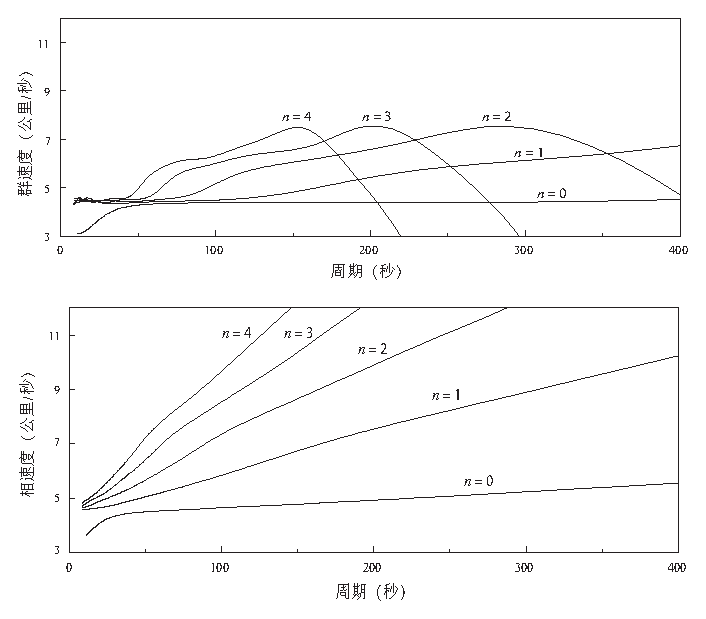
\includegraphics{../figures/chap11/fig05.eps}
}
\end{center}
\caption[Love speeds]{
\label{fig:11.5}
勒夫波的群速度$aC$({\em 上图\/})和相速度 $ac$({\em 下图\/})。
整数$n=0$和$n=1$--4分别表示基阶和前四个径向高阶分支。
当周期小于$2\pi/\omega\approx 40$~秒时,由于球对称平均的PREM模型中地壳的结构是百分之七十的海洋和百分之三十的大陆的独特的混合体,这里所展示的频散与地球上任何地方的频散都不一样。}
\end{figure}
其中$c=\om\hspace{-0.2 mm}/\hspace{-0.2 mm}k$是勒夫波的相速度。
关系式~(\ref{11.Lgrvel})的优势在于它提供了一个无需诉诸数值微分便可计算$C$的方法。

图~\ref{fig:11.5} 显示了在地球表面$r=a$上基阶($n=0$)和前四个径向高阶模式($n=1\hspace{0.2 mm}$--$\hspace{0.2 mm}4$)勒夫波的群速度$aC$和相速度$ac$作为周期$2\pi/\om$的函数的变化。
周期大于~40秒的基阶勒夫波以相对恒定的群速度$aC\approx 4.4$ 公里/秒传播。
这就解释了G波的频散相对不明显或有些脉冲讯号的特征,我们将在第~\ref{11.sec.wiggly}节中看到这一现象。
长周期的G波群绕行地球一周大约需要两个半小时。
长周期高阶模式群速度的减小是地球液态外核存在的表现;
相应的$n=2,3,4$波群震相与${\rm ScS}_{\rm SH}$是等价的,因此它们不是真正的面波。
\index{Love wave|)}%
\index{surface wave!Love|)}%

%\subsection{Rayleigh waves}
\subsection{瑞利波}
\index{Rayleigh wave|(}%
\index{surface wave!Rayleigh|(}%

控制瑞利波传播作用量的径向积分~(\ref{8.spheract}) 和~(\ref{8.Iprime})可以写为
\eq \label{11.RayI}
\sI=\half(\om^2I_1-m^2I_2-kI_3-I_4),
\en
\eq \label{11.Raylin16}
\sI'=\half(\om^2I_1-k^2I_2^{\prime}-kI_3^{\prime}-I_4^{\prime}),
\en
其中
\eq
I_1=\int_0^a\rho (U^2+V^2)\,r^2dr,
\en
\eq \label{11.Rint2}
I_2=\int_0^a[\mu\hspace{0.2 mm}U^2+(\kappa+\fourthirds\mu)V^2]\,dr,
\en
\eqa
\lefteqn{I_3=\int_0^a[\fourthirds\mu V
(\dU-r^{-1}U)-2\kappa V(\dU+2r^{-1}U)} \nonumber \\
&&\qquad\mbox{}+2\mu\hspace{0.2 mm}U(\dV-r^{-1}V)+\rho(VP+2gUV)]\,rdr,
\ena
\eqa
\lefteqn{I_4=\int_0^a[(\kappa(\dU+2r^{-1}U)^2
+\fourthirds\mu(\dU-r^{-1}U)^2} \nonumber \\
&&\qquad\mbox{}+\mu(\dV-r^{-1}V)^2 \nonumber
-2\mu r^{-2}V^2
\ena
\eq \label{11.Rint4}
\qquad\qquad\qquad+\rho(4\pi G\rho\hspace{0.3 mm}U^2
+U\dP-4r^{-1}gU^2)]\,r^2dr,
\en
\eq \label{11.need1in16}
I_2^{\prime}=I_2+\frac{1}{4\pi G}\int_0^{\infty}
P^2\,dr,
\en
\eq \label{11.need2in16}
I_3^{\prime}=I_3+\int_0^a\rho V\hspace{-0.2 mm}P\,rdr,
\en
\eq \label{11.need3in16}
I_4^{\prime}=I_4+\int_0^a\rho\hspace{0.2 mm}U\hspace{-0.2 mm}\dot{P}\,r^2dr
+\frac{1}{4\pi G}\int_0^{\infty}\dot{P}^2\,r^2dr.
\en
类似于方程~(\ref{11.tordisp}),瑞利波的能量均分或频散关系$\sI=\sI'=0$为
\index{Rayleigh-wave dispersion}%
\index{dispersion!Rayleigh-wave}%
\eq \label{11.Raydisp}
\om^2I_1-k^2I_2-kI_3-I_4=
\om^2I_1-k^2I_2^{\prime}-kI_3^{\prime}-I_4^{\prime}=0.
\en
瑞利波的能量~(\ref{8.TOTSPHEN})可以表示为
\index{energy!Rayleigh-wave}%
\index{Rayleigh-wave energy}%
\eq
\sE=\half(\om^2I_1+k^2I_2+kI_3+I_4)=
\half(\om^2I_1+k^2I_2^{\prime}+kI_3^{\prime}+I_4^{\prime}).
\en
利用频散关系式~(\ref{11.tordisp}) 和~(\ref{11.Raydisp}),
勒夫或瑞利波的总能量等于其动能的两倍,即$\sE=\om^2I_1$。

通过考虑角频率为$\om$和$\om+\delta\om$、波数为$k$和$k+\delta k$以及
径向本征函数为$U$、$V$、$P$和$U+\delta U$、$V+\delta V$、$P+\delta P$的两个波,
并且同第~\ref{11.sec.LoveC}节中一样利用瑞利原理,
我们得到类似于~(\ref{11.Lgrvel})的瑞利波群速度的解析表达式:
\index{group speed!Rayleigh-wave}%
\index{Rayleigh-wave group speed}%
\eq
C=\frac{I_2^{\prime}+\half k^{-1}I_3^{\prime}}{cI_1}.
\label{11.Rgrvel}
\en
在得到~(\ref{11.Rgrvel})这一结果时,最简单的做法是将势函数微扰$P$视为一个自变量;
而在对不带撇号的作用量$\sI$做变分时,必须考虑$P$对波数$k$的依赖性。
习惯的做法是使用~(\ref{11.Lgrvel}) 和~(\ref{11.Rgrvel})这两个关系式来定义自由振荡或驻波的群速度,
包括那些并不与面波等价的$n\ll l/4$的模式${}_n{\rm T}_l$和${}_n{\rm S}_l$。
在数学上,以这种方式定义的${}_nC_l$为经过离散本征频率$\ldots,{}_{n-1}\om_l,\,{}_n\om_l,\,{}_{n+1}\om_l,\ldots$的平滑频散曲线的斜率。
我们将在第12章得到体波等价模式的群速度的一个物理解释。

图~\ref{fig:11.6}显示了基阶($n=0$)和前四个径向高阶模式($n=1\hspace{0.2 mm}$--$\hspace{0.2 mm}4$)瑞利波频散分支的群速度$aC$和相速度$ac$作为周期的函数的变化。
\begin{figure}[!t]
\begin{center}
\scalebox{0.95}{
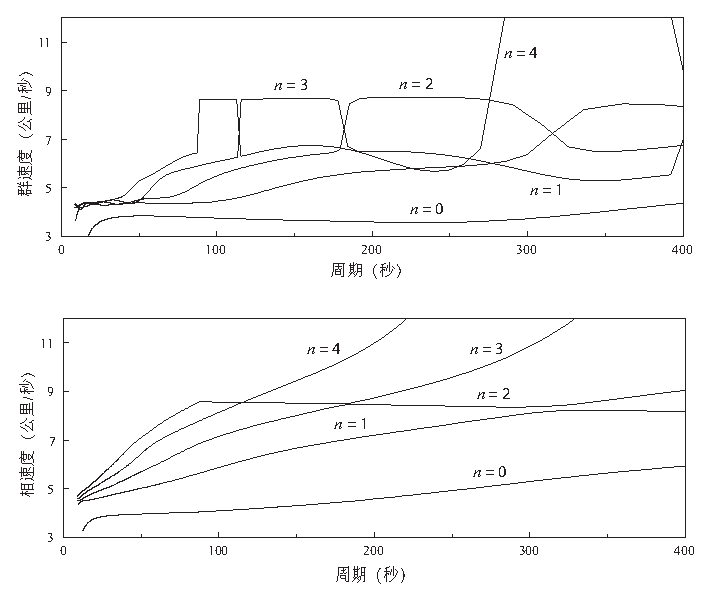
\includegraphics{../figures/chap11/fig06.eps}
}
\end{center}
\caption[Rayleigh speeds]{
\label{fig:11.6}
基阶($n=0$)和前四个径向高阶($n=1\hspace{0.2 mm}$--$\hspace{0.2 mm}4$)瑞利波的群速度$aC$({\em 上图\/})与相速度$ac$({\em 下图\/})。
在周期大于$2\pi/\omega\approx 200$秒时群速度曲线的分段线性特征是由于采样不足而造成的假象。
当周期小于$2\pi/\omega\approx 40$~秒时,由于球对称平均的PREM模型中地壳的结构是百分之七十的海洋和百分之三十的大陆的独特的混合体,这里所展示的频散与地球上任何地方的频散都不一样。
}
\end{figure}
在PREM模型中,基阶瑞利波的群速度在周期$2\pi/\om\approx 240$秒有一个范围较大的局部极小值$aC_{\rm min}\approx 3.6$~公里/秒,而在周期$2\pi/\om\approx 50$ 秒
则有一个范围较大的局部极大值$aC_{\rm max}\approx 3.8$~公里/秒。
速度最快的波是穿透到上地幔较深部高速区域的很长周期的波;
当周期约为300秒时,群速度$aC$会超过~3.8 公里/秒。
周期为50--300秒的基阶瑞利波群的传播速度会比同周期段的基阶勒夫波群稍慢一些;
这些长周期的基阶瑞利波几乎需要三个小时才能绕行地球一周,比准单频的G波多用半小时。
$n=1,2,\ldots$与$n=0$群速度之间的明显的不同使我们能够容易地通过在时间域中加窗来将较单纯的基阶瑞利波群与较早到达的高阶模式分离开来。
而$n=1,2,\ldots$和$n=0$的勒夫波群则更接近同时到达,
特别是在周期小于100--150~秒时(见图~\ref{fig:11.5})。
因此,基阶勒夫波频散的测量比基阶瑞利波的测量更容易被高阶模式的干扰污染。

横跨$ac\approx 8.6$~公里/秒的几乎为常数的相速度曲线是核幔边界Stoneley模式分支,它与瑞利波的高阶模式紧密地交织在一起。
\index{Stoneley mode}%
\index{mode!Stoneley}%
群速度的奇特的陡增和$aC\approx 8.6$~公里/秒的群速度高地也是同一现象的表现;
Stoneley模式相速度与群速度的一致性是其无频散特性的必然结果。
在大多数情形下,例如$n=3\hspace{0.2 mm}$--$\hspace{0.2 mm}4$之间在约120秒处急剧地回避相交,可以简单的将Stoneley模式除去,然后重新指定瑞利波的阶数。 
然而,对于$n=2\hspace{0.2 mm}$--$\hspace{0.2 mm}3$之间的渐变,特别是$n=1\hspace{0.2 mm}$--$\hspace{0.2 mm}2$之间的密切式特征,这样的做法就有点草率了。
在使用~(\ref{10.appacc}) 式或~(\ref{11.accsum})式来合成球对称地球上的面波加速度图时,
最好是简单地在对各阶模式的叠加中保Stoneley分支;
当然,由于源点和接收点都远在相应本征函数的指数衰减的尾端,因此Stoneley模式对响应的贡献很小。
\index{Rayleigh wave|)}%
\index{surface wave!Rayleigh|)}%

\renewcommand{\thesubsection}{$\!\!\!\raise1.3ex\hbox{$\star$}\!\!$
\arabic{chapter}.\arabic{section}.\arabic{subsection}}
%\subsection{Tsunamis}
\subsection{海啸}
\index{tsunami|(}%
\renewcommand{\thesubsection}{\arabic{chapter}.\arabic{section}.\arabic{subsection}}

在第8.8.11节中,我们指出像PREM这样的有海洋覆盖的地球模型是支持海啸模式的,
其球型位移本征函数$U,V$主要局限于地表的液态层。
图\ref{fig:11.7}显示了在水深为$h=2$公里、$h=4$公里和$h=6$公里时,
这些模式的相速度和群速度作为周期的函数。
对每一深度,相应的振荡的球谐函数次数~$l=10$, $l=100$ 和 $l=1000$ 都在图的最顶上给出。
\begin{figure}
\begin{center}
\scalebox{0.9}{
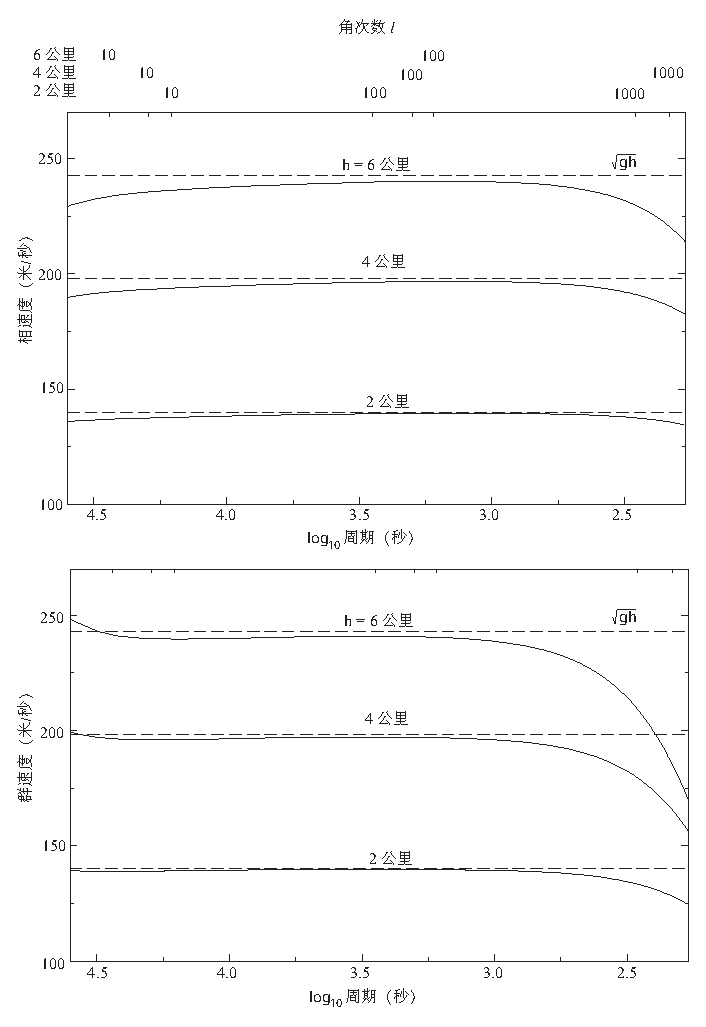
\includegraphics{../figures/chap11/fig07.eps}
}
\end{center}
\caption[tsunami speeds]{
\label{fig:11.7}
修改后的地表海水深度为$h=2$~公里、$h=4$~公里 或 $h=6$~公里的PREM模型中海啸模式的相速度 $ac$({\em 上图\/})与群速度 $aC$({\em 下图\/})。
虚线表示无频散的浅水表面重力波的恒定速度$ac=aC=\sqrt{gh}$,以供比较。}
\end{figure}
覆盖在刚性海床之上的海洋中其表面重力波相速度和群速度的经典结果为(Lamb \citeyear{lamb32};
\citeyear{lighthill78})
\index{phase speed!tsunami}%
\index{group speed!tsunami}%
\eq \label{11.classical}
ac=\sqrt{gk^{-1}\,{\rm tanh}\,kh},\qquad
aC=\half ac\left(1+\frac{2kh}{{\rm sinh}\,2kh}
\right).
\en
在浅水极限$kh\ll 1$下,
\index{shallow-water limit}%
表面重力波的传播是无频散的,
\eq \label{classical2}
ac=aC=\sqrt{gh},
\en
而在深水极限$kh\gg 1$下,相速度是群速度的两倍,
\eq
ac=2aC=\sqrt{gk^{-1}}.
\en
在周期大过1000~秒时,海啸波基本上是属于无频散的浅水波,
其速度取决于水深,约为150米/秒至250米/秒之间。
传过太平洋海盆的时间约为10小时,因此在
地震发生后有足够的时间来对高风险的沿岸地区进行疏散。
周期小于1000秒时,频散符合经典的关系式~(\ref{11.classical});
在周期很长时会偏离刚性底部极限$ac=aC=\sqrt{gh}$,这是由于海床的弹性弯曲所致。
\index{tsunami|)}%

\renewcommand{\thesubsection}{$\!\!\!\raise1.3ex\hbox{$\star$}\!\!$
\arabic{chapter}.\arabic{section}.\arabic{subsection}}
%\subsection{Transverse isotropy}
\subsection{横向各向同性}
\index{transverse isotropy!surface-wave|(}%
\renewcommand{\thesubsection}{\arabic{chapter}.\arabic{section}.\arabic{subsection}}

上述结果也适用于横向各向同性地球模型,
条件是将~(\ref{11.Lint2})--(\ref{11.Lint3})中的勒夫波径向积分改为
\eq \label{11.tiI2}
I_2=\int_0^aNW^2\,dr,
\en
\eq
I_3=\int_0^a[L(\dW-r^{-1}W)^2-2Nr^{-2}W^2]\,r^2dr,
\en
而将~(\ref{11.Rint2})--(\ref{11.Rint4})中的瑞利波的积分改为
\eq
I_2=\int_0^a[AU^2+LV^2]\,dr,
\en
\eqa
\lefteqn{I_3=\int_0^a[2LU(\dV-r^{-1}V)-2F\dU V} \nonumber \\
&&\qquad\mbox{}-4(A-N)r^{-1}UV+\rho(VP+2gUV)]\,rdr,
\ena
\eqa
\lefteqn{I_4=\int_0^a[C\dU^2+4Fr^{-1}\dU U
+4(A-N)r^{-2}U^2} \nonumber \\
&&\qquad\mbox{}+L(\dV-r^{-1}V)^2 \nonumber
-2Nr^{-2}V^2
\ena
\eq \label{11.tiI4}
\qquad\qquad\qquad+\rho(4\pi G\rho U^2+U\dP-4r^{-1}gU^2)]\,r^2dr.
\en
(\ref{11.tiI2})--(\ref{11.tiI4})中的$C$、$A$、$L$、$N$和$F$是第8.9节中所引入的五个弹性参数。
\index{transverse isotropy!surface-wave|)}%
\index{dispersion relation|)}%
\index{group speed|)}%
\index{speed!group|)}%


%\section{Surface-Wave Seismograms}
\section{面波地震图}
\index{seismogram!surface-wave|(}%
\index{surface-wave seismogram|(}%
\label{11.sec.wiggly}

面波的合成加速度图可以通过~(\ref{11.accsum})的双重求和的快速傅里叶反变换来计算。
然而,这种方法严格要求震中距的范围为$0\ll\Theta\ll\pi$。
由于该限制,更好的做法还是简单地将对应的本征模式${}_n{\rm T}_l$
和${}_n{\rm S}_l$沿每条勒夫和瑞利波频散分支$n=0,1,2,\ldots$进行叠加;
我们利用这种一致成立的方法来计算在此所展示的面波加速度图$\ba(\bx,t)$和位移地震图$\bs(\bx,t)$。

%\subsection{Mantle waves and X waves}
\subsection{地幔波和X波}
\index{mantle wave|(}%
\index{X wave|(}%

图~\ref{fig:11.15}显示了1994年10月4日千岛群岛地震事件之后,
\index{Kuril Islands 1994 earthquake}%
在澳大利亚Tasmania的TAU台站的径向、纵向和横向分量的加速度。
\begin{figure}[!b]
\begin{center}
\scalebox{0.98}{
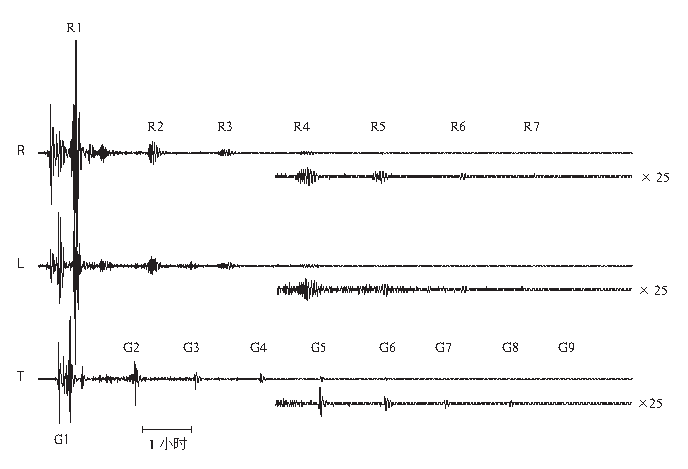
\includegraphics{../figures/chap11/fig08.eps}
}
\end{center}
\caption[multi-orbit]{
\label{fig:11.15}
合成的多周面波加速度图。
震源是1994年10月4日的千岛群岛浅源大地震;
接收点位于澳大利亚Tasmania。
每条记录都是完备的模式叠加,且在周期50到250秒之间进行了带通滤波,
以突显激发较强的基阶勒夫和瑞利波;
图中标示了径向(R)、纵向(L)和横向(T)分量以及R1--R7和G1--G9的波群讯号。
勒夫波的群速度明显较快:$aC_{\rm R}=3.6$--3.8~公里/秒,而 $aC_{\rm L}=4.4$~公里/秒。
由于非弹性衰减,周数较多的波R4--R6和G5--G8要比R1和G1弱许多;
但是如果放大25倍画出,它们便清晰可见。
}
\end{figure}
这个浅源地震大(地震矩$M_0=4\times 10^{21}$~N\hspace{0.5 mm}m)激发了
惊人的多周波列。
肉眼可见清晰的直到R6的基阶模式瑞利波讯号,
而勒夫波讯号甚至到G8都可以辨认出来。
这些叫做地幔波的长周期面波绕行地球多达四周!
\index{mantle wave}%
在地震的对跖点$\Theta=\pi$处,优弧波和劣弧波Gl、G2或R1、R2同时到达并相互干涉。 
在图~\ref{fig:11.16}中我们画出对跖点附近的瑞利波记录剖面来展示这一现象。
在这一焦点处能量的明显聚焦值得注意。
\begin{figure}
\begin{center}
\scalebox{1.05}{
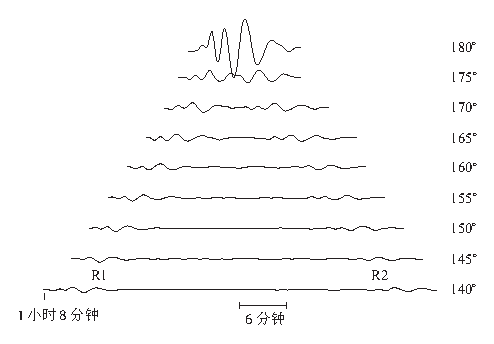
\includegraphics{../figures/chap11/fig09.eps}
}
\end{center}
\caption[Rayleigh antipode]{
\label{fig:11.16}
对跖点附近的径向分量瑞利波加速度图。
位于赤道上的假想震源的矩张量${\bf M}$与1994年10月4日的千岛群岛地震相同;
接收点也均位于赤道上,在震源正东方,震中距范围为$\Theta=140^{\circ}$至$\Theta=180^{\circ}$。所有记录均以相同比例绘制,以展示优弧和劣弧震相R1和R2在对跖点的放大。}
\end{figure}

长周期勒夫波的传播特性从图~\ref{fig:11.transrecn0}所展示的横向分量合成记录剖面中可以更清楚地辨识。
震源是一个假想的深度为300公里的走滑地震;
在横向位移地震图$\bPhih\cdot\bs(\bx,t)$的合成中仅叠加了基阶环型模式${}_0{\rm T}_l$。
源点-接受点之间几何关系的设置使得球型模式${}_n{\rm S}_l$不会被激发。
前五个到达的勒夫波讯号G1--G5很容易识别。
有两个特点值得注意:
一是波形的脉冲特性,这是由于周期大于$2\pi/\om\approx 40$~秒时近乎常数的群速度$aC\approx 4.4$~公里/秒;另外,同相位(即所有的波峰或波谷)的连线与波群整体的到达对不齐。
最适合观察后一种现象的做法是用一只眼睛靠近页面,以掠射的角度来观看这张图;
由于地幔勒夫波的相速度高于其群速度$c>C$,因此波前以微小的夹角超越波群。
图~\ref{fig:11.transrec} 显示了相同的$\bPhih\cdot\bs(\bx,t)$记录剖面,
但在叠加中除了环型的基阶模式${}_0{\rm T}_l$外,也包含了高阶的${}_1{\rm T}_l,{}_2{\rm T}_l,\ldots$。
由于高阶模式群速度较高,因此它们比基阶模式的G波先到。
可以识别对应于直达和多次反射的${\rm SH},{\rm SS}_{\rm SH},{\rm SSS}_{\rm SH},\ldots$体波的清楚的震相。
还要注意的是在地核阴影边界$\Theta\approx 100^{\circ}$之外衍射SH波的
振幅呈指数衰减。

\begin{figure}
\begin{center}
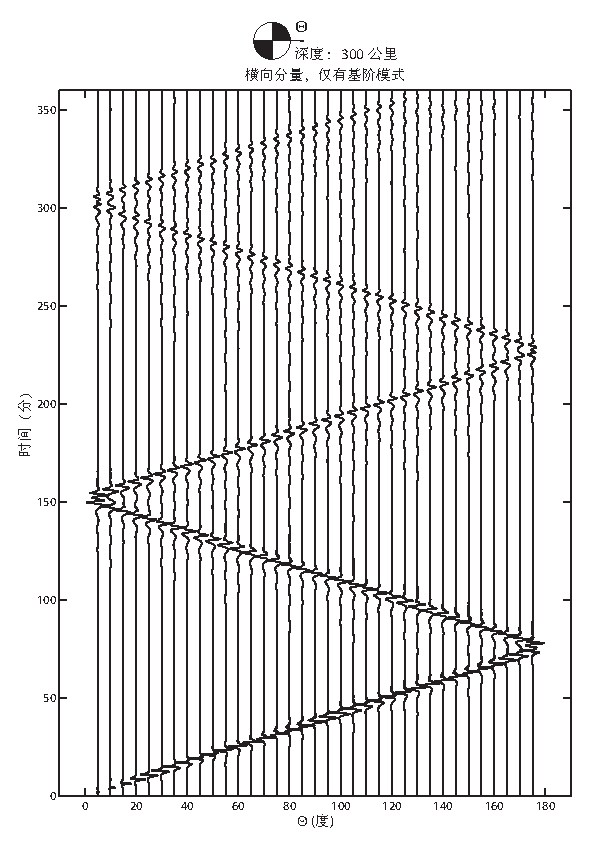
\includegraphics{../figures/chap11/fig10.eps}
\end{center}
\caption[transverse record sections n=0]{
\label{fig:11.transrecn0}
PREM地球模型中一个深度为300公里且具有脉冲震源时间函数$\dot{m}(t)$的走滑断层所产生的基阶模式横向分量位移$\hat{\bf \Phi}\cdot{\bf s}({\bf x},t)$地震图记录剖面。
最上方为地震震源机制示意图;
沙滩球的黑白区域分别对应于下半震源球面上P波压缩和膨胀的象限。
台站均在震源的正东方(如沙滩球上的箭头所示),震中距$\Theta$间隔为$5^\circ$的位置上。
}
\end{figure}

图~\ref{fig:11.radialsecn0}和\ref{fig:11.radialsec}显示了同一个
300公里深的走滑地震事件的合成径向分量位移$\brh\cdot\bs(\bx,t)$地震图,分别是叠加球型基阶模式${}_0{\rm S}_l$和基阶加高阶模式${}_1{\rm S}_l,{}_2{\rm S}_l,\ldots$而得到的。
基阶模式瑞利波的传播的频散特征很明显:
在每个R1--R4讯号中,最早和最晚到的波的周期分别为$2\pi/\om\approx 50$~秒和$2\pi/\om\approx 240$~秒;
它们是与瑞利波群速度的两个极值$aC_{\rm max}\approx 3.8$~公里/秒
和$aC_{\rm min}\approx 3.6$~公里/秒相应的艾利震相。
同勒夫波的情形一样,因为地幔瑞利波的相速度大于群速度,所有的波峰和波谷都走得比波群本身快。
同样地,最容易辨识这一相位和波群到达对不齐的现象还是采用“比目鱼眼"的视角。

\begin{figure}[!t]
\begin{center}
\scalebox{1.0}{
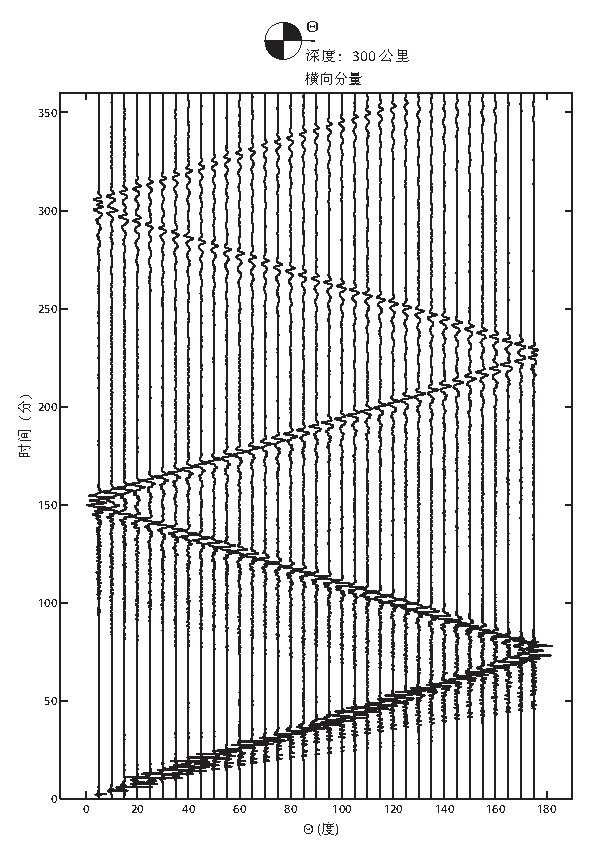
\includegraphics{../figures/chap11/fig11.eps}
}
\end{center}
\caption[transverse record sections]{
\label{fig:11.transrec}
与图~\ref{fig:11.transrecn0}相同,但此处包含了高阶模式的勒夫波。
计算合成地震图时叠加了所有频率低于 50 mHz的环型多态模式${}_n{\rm T}_l$。
图中可见速度较快的高阶模式讯号。
}
\end{figure}
\begin{figure}
\begin{center}
\scalebox{0.95}
{
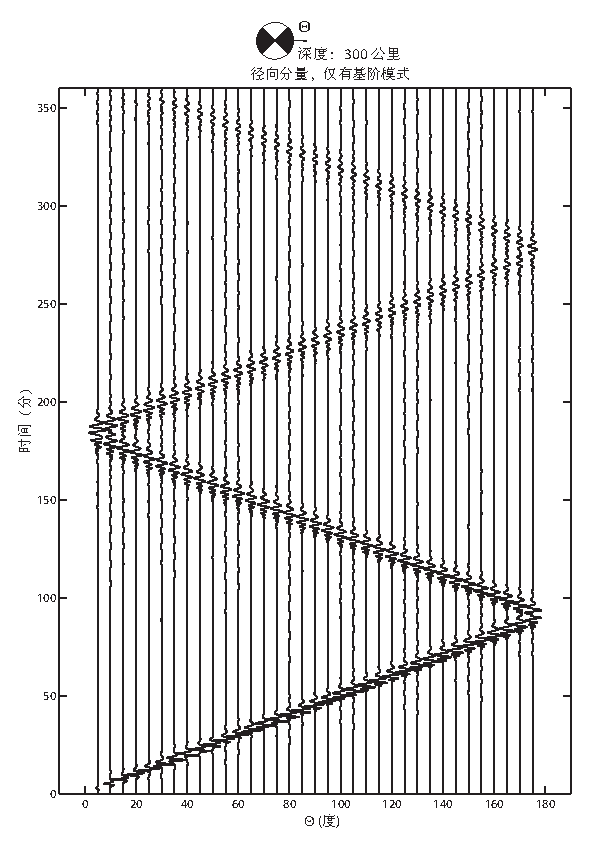
\includegraphics{../figures/chap11/fig12.eps}
}
\end{center}
\caption[radial record sections n=0]{
\label{fig:11.radialsecn0}
PREM地球模型中一个深度为300公里且具有脉冲震源时间函数$\dot{m}(t)$的走滑断层所产生的基阶模式径向分量位移$\hat{\bf r}\cdot{\bf s}({\bf x},t)$地震图记录剖面。
最上方为地震震源机制示意图;
沙滩球的黑白区域分别对应于下半震源球面上P波压缩和膨胀的象限。
台站均在震源的正东方(如沙滩球上的箭头所示),震中距$\Theta$间隔为$5^\circ$的位置上。源点-接受点之间几何关系的设置,包括显示的走向为N$45^{\circ}$E的断层,确保环型模式${}_n{\rm T}_l$不会被激发。
}
\end{figure}
\begin{figure}[!t]
\begin{center}
\scalebox{0.95}
{
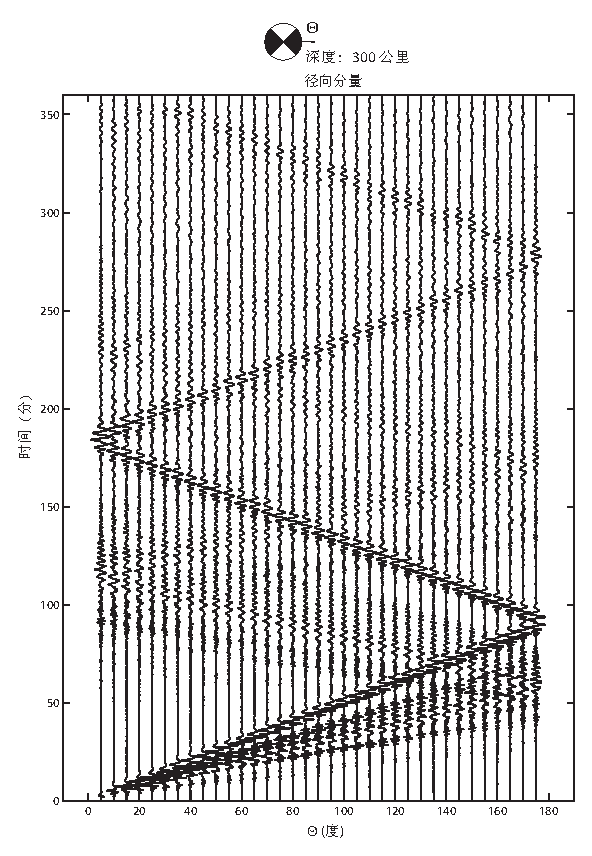
\includegraphics{../figures/chap11/fig13.eps}
}
\end{center}
\caption[radial record section]{
\label{fig:11.radialsec}
与图~\ref{fig:11.radialsecn0}相同,但此处包含了高阶模式的瑞利波。
这些$aC=5\!-\!7$~公里/秒的波的叠加被称为X震相。
计算合成地震图时叠加了所有频率低于50 mHz的所有球型多态模式${}_n{\rm S}_l$。
}
\end{figure}
在R1--R4之前到达的高阶模式震相要比勒夫波的情形更加明显;
这些长周期的高阶瑞利波的群速度介于$aC=5\!-\!7$~公里/秒之间。
它们在大地震后的径向和纵向宽频记录中普遍存在这一现象是Jobert, Gaulon, Dieulin \& Roult (\citeyear{jobert&al77})最先指出的。
这些学者准确地认识到这些高速震相是“球型谐波的叠加(une superposition d'harmoniques sph\'{e}ro\"{\i}daux)”;
尽管如此肯定,他们还是不可思议地将其命名为{\em X波\/}。
\index{X wave}%
在合成的记录剖面中,可以追踪到绕行地球数周的复杂的多个模式的X波群;
与其等效的体波震相包括SV在地表的多次反射以及每次反射所产生的SV到P的转换波。

\begin{figure}
\begin{center}
\scalebox{0.9}
{
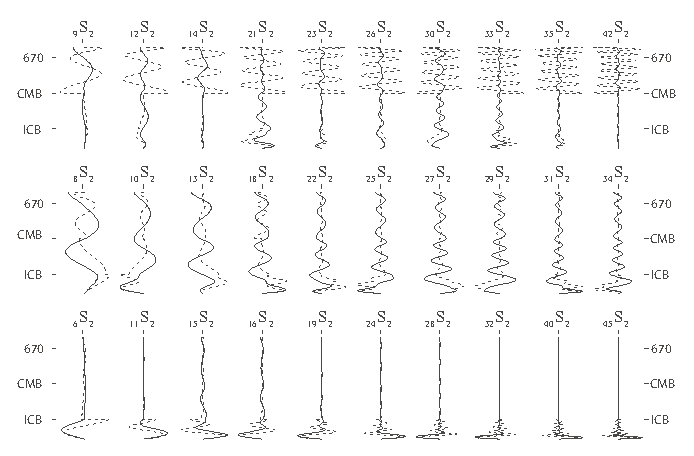
\includegraphics{../figures/chap11/fig14.eps}
}
\end{center}
\caption[Shearer stack]{
\label{fig:11.shearer}
IDA地震台网在1981--1991这11年间所记录到的径向分量加速度图$\hat{\bf r}\cdot{\bf a}({\bf x},t)$的叠加记录剖面。
({\em 左图\/})地震后$t=0\!-\!3$小时时段。({\em 右图\/})地震后$t=3\!-\!6$小时时段。
绘图方式是地震反射勘探行业中普遍使用的:正负振幅分别为黑白颜色。
每个叠加的加速度图都缩放为在前100分钟内有相同的均方根振幅。
这里对多周震相通过乘以一个增益调整因子$\sqrt{t}$进行了加强,与图~\ref{fig:11.transrecn0}--\ref{fig:11.radialsec}中显示的一样。
(由P. Shearer提供)。
}
\end{figure}
\begin{figure}
\begin{center}
\scalebox{0.9}
{
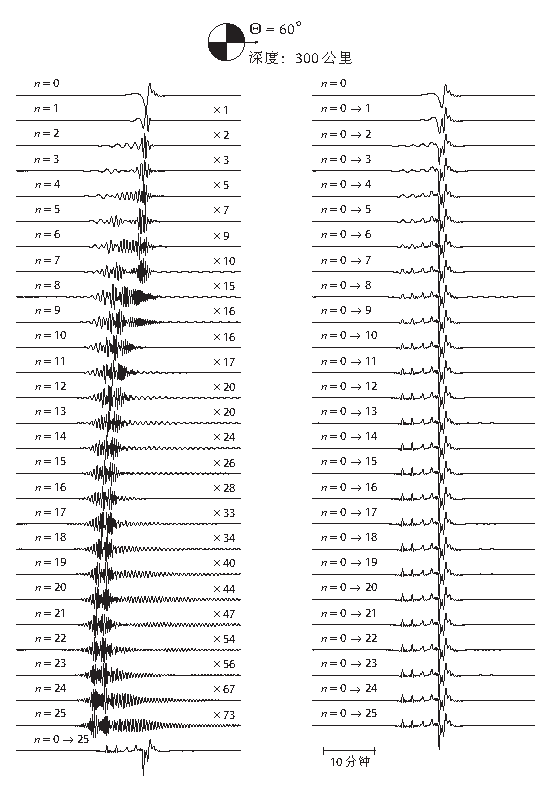
\includegraphics{../figures/chap11/fig15.eps}
}
\end{center}
\caption[overtonesL]{
\label{fig:15.overtonesL}
一个中等深度($h=300$~km)走滑断层的横向分量位移响应$\hat{\bf \Phi}\cdot{\bf s}({\bf x},t)$。
({\em 顶图\/})震源机制和源点-接收点几何关系示意图。
({\em 左图\/})基阶和前25个高阶环型模式分支对地震图的贡献,从最上方的$n=0$开始,到最下方之上的$n=25$。图中标示了每个高阶分支的放大因子;
例如,这里所画的$n = 10$分支地震图相对于基阶模式地震图放大了16倍。
最下方显示的是$n=0\!\rightarrow\!25$的完整的合成地震图。 
({\em 右图\/})每增加一个分支的累加效果。
最上方的地震图只包括基阶($n=0$)模式,第二个显示的是增加第一个高阶模式的效果,
而第三个则包括$n=0\!\rightarrow\!2$的分支,以此类推。
最后一道仍然是$n=0\!\rightarrow\!25$的完整的合成地震图。
}
\end{figure}
\begin{figure}
\begin{center}
\scalebox{0.95}
{
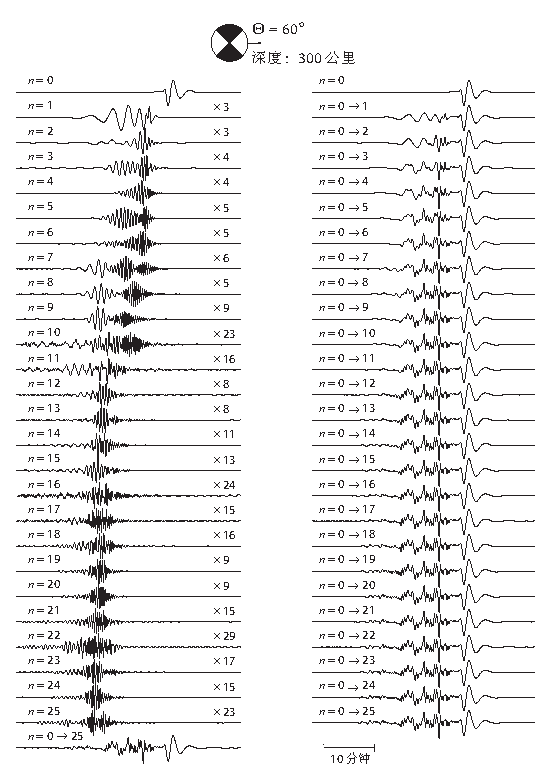
\includegraphics{../figures/chap11/fig16.eps}
}
\end{center}
\caption[overtonesR]{
\label{fig:15.overtonesR}
一个深度为$300$~km的走滑断层的径向分量位移响应$\hat{\bf r}\cdot{\bf s}({\bf x},t)$。
({\em 顶图\/}) 震源机制和源点-接收点几何关系示意图。
({\em 左图\/})基阶和前25个高阶球型模式分支对地震图的贡献,从最上方的$n=0$开始,到最下方之上的$n=25$。图中标示了每个高阶分支的放大因子;
例如,这里所画的$n = 10$分支地震图相对于基阶模式地震图放大了23倍。
最下方显示的是$n=0\!\rightarrow\!25$的完整的合成地震图。 
({\em 右图\/})每增加一个分支的累加效果。
最上方的地震图只包括基阶($n=0$)模式,第二个显示的是增加第一个高阶模式的效果,
而第三个则包括$n=0\!\rightarrow\!2$的分支,以此类推。
最后一道仍然是$n=0\!\rightarrow\!25$的完整的合成地震图。
}
\end{figure}
\begin{figure}[!t]
\begin{center}
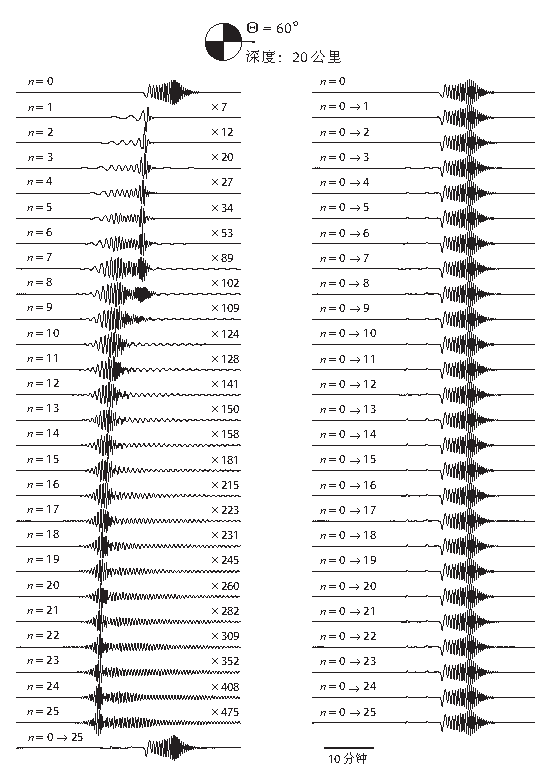
\includegraphics{../figures/chap11/fig17.eps}
\end{center}
\caption[overtonesL2]{
\label{fig:15.overtonesL2}
与图~\ref{fig:15.overtonesL}相同,但震源为浅源($h=20$~公里)走滑地震。
注意这里高阶的放大因子大很多,表明基阶($n=0$)模式占主导地位。
}
\end{figure}
\begin{figure}[!t]
\begin{center}
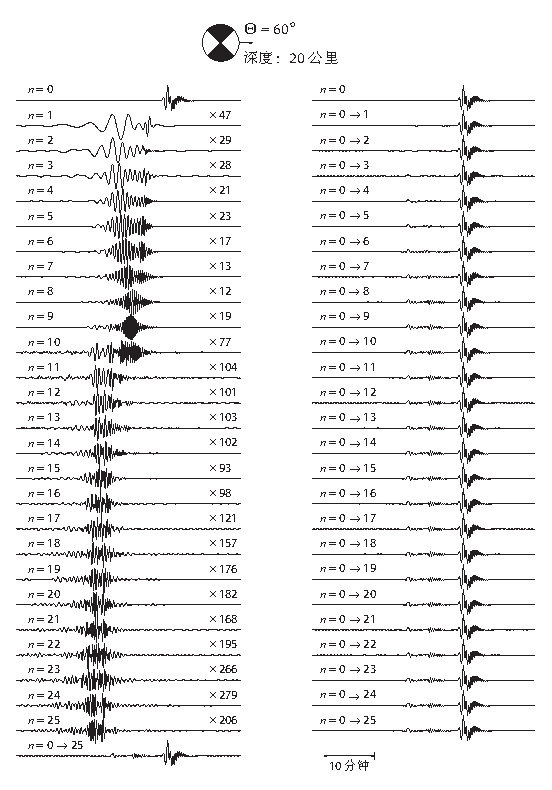
\includegraphics{../figures/chap11/fig18.eps}
\end{center}
\caption[overtonesR2]{
\label{fig:15.overtonesR2}
与图~\ref{fig:15.overtonesR}相同,但震源为浅源($h=20$~公里)走滑地震。
注意这里高阶的放大因子大很多,表明基阶($n=0$)模式占主导地位。
}
\end{figure}
在上述四个记录剖面中所画的是$\sqrt{t}\times\bs(\bx,t)$这一乘积,而并非原始的质点位移$\bs(\bx,t)$。
这一时间平方根的增益调整会增强晚到的震相,使它们更容易看清楚。
图~\ref{fig:11.shearer}显示了在叠加的径向加速度图中,
X震相以及基阶模式瑞利波相位和波群到达对不齐的现象都很明显;
这种黑白的绘图方式加上$\sqrt{t}$的增益调整给我们带来一个地球的长周期面波响应
在整个展示的$0^{\circ}\leq\Theta\leq 180^{\circ}$距离
和 $0\leq t\leq 6$~小时时间范围内都是相当均匀的视觉图像
(Shearer \citeyear{shearer94a})。

在图~\ref{fig:15.overtonesL} and~\ref{fig:15.overtonesR}中,
我们剖析了震中距$\Theta=60^{\circ}$处的优弧勒夫和瑞利波响应$\bPhih\cdot\bs(\bx,t)$和 $\brh\cdot\bs(\bx,t)$,
来展示单独的环型和球型模式分支${}_0{\rm T}_l$\hspace{0.3 mm}--\hspace{0.3 mm}${}_{25}{\rm T}_l$
和 ${}_0{\rm S}_l$\hspace{0.3 mm}--\hspace{0.3 mm}${}_{25}{\rm S}_l$的相对贡献。
与前面一样,假想的震源还是深度为300公里的走滑断层。
每个图的左侧一列显示的是单一分支的地震图,而右侧一列则为累积的分支叠加;
该绘图方式可以详细揭示${\rm SH},{\rm SS}_{\rm SH},{\rm SSS}_{\rm SH},\ldots$这些体波和
组成X震相的SV和P-SV多次反射波是如何在$n=1,2,\ldots$这些高阶分支叠加的过程中,被慢慢构筑起来的。
图~\ref{fig:15.overtonesL2} 和~\ref{fig:15.overtonesR2}显示了
浅源($h=20$~公里)走滑震源响应中将一个个分支剥离后的效果。
在这个例子中,基阶模式${}_0{\rm T}_l$ 和 ${}_0{\rm S}_l$对地震图的贡献是占主导地位的。
勒夫波列起始时有如脉冲的讯号是群速度为$aC\approx 4.4$~公里/秒的G波;
其高度频散的尾巴,则是由被围陷在24.4公里厚的PREM地壳中速度较慢慢、周期较短($2\pi/\om<40$~秒)的波所组成。
径向分量地震图的尾巴同样也是由短周期的地壳瑞利波组成。
这些短周期的波都不会被中等深度($h=300$~公里)的震源所强烈激发。
\index{mantle wave|)}%
\index{X wave|)}%

\begin{figure}[!b]
\begin{center}
\scalebox{0.98}{
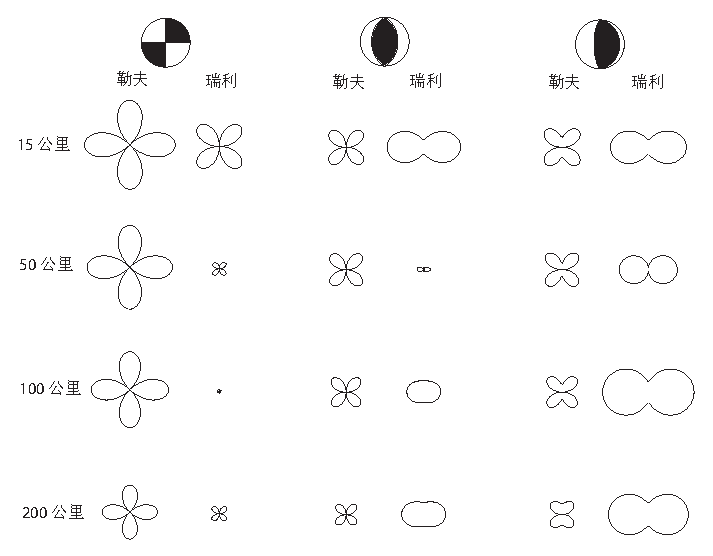
\includegraphics{../figures/chap11/fig19.eps}
}
\end{center}
\caption[L&R rad pats]{
\label{fig:11.8}
走滑断层({\em 左图\/})、$45^{\circ}$ 倾角的逆冲断层({\em 中图\/})以及低角度逆冲或高倾角正断层({\em 右图\/})
所辐射的勒夫波和瑞利波在不同方向的振幅。
相关的震源机制显示于图的上方;其下的几行呈现了极座标中深度为$h=15$--200公里的震源的辐射花样$|R(\Phi)|$。所有图中波的周期均为$2\pi/\omega=100$~秒;
且所有花样均用相同的比例绘制。}
\end{figure}


%\subsection{Effect of source mechanism}
\subsection{震源机制的影响}
\label{11.sec.radpat}

在图~\ref{fig:11.8}中,我们展示了多种理想化的震源机制和震源深度$h=a-r_{\rm s}$的
面波辐射随方位的变化。
其中显示了100秒的基阶勒夫和瑞利波辐射花样的模数$|R(\Phi)|$;
这一{\em radiation
辐射振幅\/}
\index{radiation amplitude}%
\index{amplitude!radiation}%
对于任意矩张量震源都是方位角的偶函数:
\eq 
|R(\Phi)|=|R(\Phi+\pi)|.
\en
\begin{figure}[!b]
\begin{center}
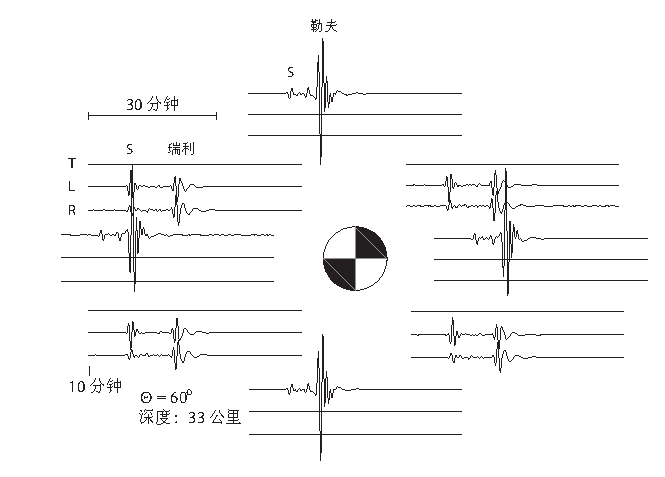
\includegraphics{../figures/chap11/fig20.eps}
\end{center}
\caption[surface seismo1]{
\label{fig:11.9}
辐射花样$R(\Phi)$对于面波加速度图的影响。
震源是位于$h=33$~公里深度的垂直走滑断层;
图中央的沙滩球中黑白区域分别对应下半震源球上P波的压缩和膨胀的象限。
接收点位于地震的({\em 从最上方按顺时针方向\/})北方、东北方、东方、东南方、南方、西南方、西方和西北方,
震中距均为$\Theta=60^{\circ}$。
图中标示了横向(T)、纵向(L)和径向(R)分量以及S波、勒夫波和瑞利波讯号。
与图~\protect\ref{fig:10.18}相同,只是这里将模式叠加结果带通滤波到20至250秒周期,以便更加凸显面波。}
\end{figure}
另外要注意的是,由于在$\bM\rightarrow -\bM$这一替换下绝对值$|R(\Phi)|$是不变的,
因此,由图示的震源机制或者将沙滩球中黑白象限互相交换的机制所产生的辐射花样是一样的;例如,中间一列可表征$45^{\circ}$倾角的逆冲断层或者$45^{\circ}$倾角的正断层。

\begin{figure}[!b]
\begin{center}
\scalebox{1.04}{
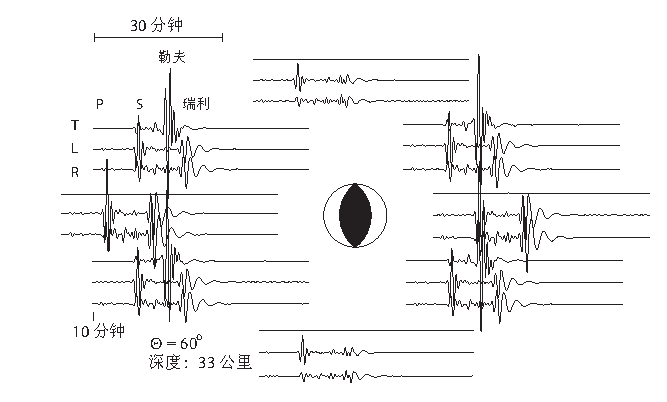
\includegraphics{../figures/chap11/fig21.eps}
}
\end{center}
\caption[surface seismo2]{
\label{fig:11.10}
与图Figure~\protect\ref{fig:11.9}相同,但震源为浅源($h=33$~公里)逆冲断层。
图中标示了横向(T)、纵向(L)和径向(R)分量以及S波、勒夫波和瑞利波讯号。
这是图~\protect\ref{fig:10.19}的面波版本。}
\end{figure}

对于一个纯粹的垂直走滑地震,矩张量分量中仅有$M_{\theta\theta}$、 $M_{\phi\phi}$和$M_{\theta\phi}$是非零的。 
因此勒夫和瑞利波的辐射花样$|R(\Phi)|$均表现出纯粹的四极$\sin2\Phi$、
$\cos2\Phi$依赖性;
在平行和垂直断层走向的方向上勒夫波的最大值与瑞利波辐射花样方位上的节点重合,反之亦然。
勒夫波的辐射强度随震源深度的增加而单调下降;
这直接反映了本征函数$W_{\rm s}$的近指数衰减(见图~\ref{fig:Lovemodes2})。
而切向瑞利波本征函数$V_{\rm s}$在$h\approx 100$~公里处有一个节点(见图~\ref{fig:fundsphmodes});
正因为如此,在这一深度上没有任何100~秒的瑞利波能够被走滑断层激发。
更短和更长周期的瑞利波对走滑断层分别在更浅和更深的地方有类似的节点。
由理想化的逆冲和正断层所激发的勒夫波也表现出占主导地位的四极辐射花样;
而瑞利波则表现出一种各向同性结合双极的辐射花样。
要注意的是,一个双力偶震源是可以没有方位上的节点的:
一个深度为100~公里、倾角为$45^{\circ}$的断层的100~秒瑞利波辐射是非常接近各向同性的。
在浅部,勒夫和瑞利波辐射的最小值都与逆冲或正断层的B轴重合。

图~\ref{fig:11.9}和~\ref{fig:11.10} 分别显示了由走滑断层和$45^{\circ}$倾角的逆冲断层所激发的勒夫波和瑞利波加速度图。
绘图方式与图~\ref{fig:10.18} 和~\ref{fig:10.19}相同,只是为了凸显基阶面波,
将模式叠加结果带通滤波到20至250秒周期, 而不是20至80~秒。
在走滑断层的例子中,勒夫波在东北、东南、西南和西北方向的节点,以及瑞利波在北、东、南和西方向的节点显而易见。还要注意的是逆冲断层的勒夫波在北、东、南和西方向的节点以及瑞利波没有任何节点但东西方向上的辐射占主导地位。
\index{seismogram!surface-wave|)}%
\index{surface-wave seismogram|)}%

%\section{Surface-Wave Perturbation Theory}
\section{面波微扰理论}
\index{surface-wave perturbation theory|(}%
\index{perturbation!surface-wave|(}%
\label{11.sec.cpert}

(\ref{eq:9.delomiso})和~(\ref{eq:9.delomiso2})两式给出了球对称各向同性微扰
$\delta\hspace{-0.1 mm}\kappa$、$\delta\hspace{-0.2 mm}\mu$、
$\delta\hspace{-0.2 mm}\rho$、$\delta\hspace{-0.1 mm}d$ 
或
$\delta\hspace{-0.1 mm}\alpha$、$\delta\hspace{-0.2 mm}\beta$、
$\delta\hspace{-0.2 mm}\rho$、$\delta\hspace{-0.1 mm}d$ 
对自由振荡或驻波的本征频率${}_n\om_l$的一阶效应。
同样地,(\ref{eq:9.delomti}) 和~(\ref{eq:9.delomti2})两式给出了横向各向同性微扰
$\delta C$, $\delta\hspace{-0.2 mm}A$、
$\delta\hspace{-0.1 mm}L$、$\delta\hspace{-0.1 mm}N$、
$\delta\hspace{-0.1 mm}F$ 
或
$\delta\hspace{-0.1 mm}\alpha_{\rm v}$、
$\delta\hspace{-0.1 mm}\alpha_{\rm h}$、
$\delta\hspace{-0.2 mm}\beta_{\rm v}$、
$\delta\hspace{-0.2 mm}\beta_{\rm h}$、$\delta\eta$
的效应。
如果我们将扰动后地球模型上的行波频散关系表示为
\eq \label{11.omofk}
\om=\om_n(k)+\delta\om_n(k),
\en
那么就可以用这些表达式来得到对于{\em 固定的波数\/}$k$,在第$n$个径向高阶分支上波的角频率变化$\delta\om_n(k)$。
由于定量的面波分析是在频率域中进行的,因此最好将~(\ref{11.omofk})改写为
\eq \label{11.kofom}
k=k_n(\om)+\delta k_n(\om),
\en
同时改为考虑对于{\em 固定角频率\/}$\om$的波数变化$\delta k_n(\om)$。
将扰动后的频散关系式~(\ref{11.omofk})在扰动前的波数$k_n(\om)$附近展开,
可以很容易地得到$\delta k_n(\om)$和$\delta\om_n(k)$这两个微扰之间的一阶关系:
\eq \label{11.omofk2}
\om=\om_n(k_n)+C_n(k-k_n)+\delta\om_n(k_n)+\cdots,
\en
其中$C_n=d\om_n/\hspace{-0.2 mm}dk$为群速度。
因为扰动前的地球上的频散关系为$\om=\om_n(k_n)$,
(\ref{11.omofk2})的左边与其右边的第一项相互抵消。
因此,在波数的一阶变化$\delta k_n=k-k_n$为
\index{perturbation!wavenumber}%
\eq \label{11.twoperts}
\delta k=-C^{-1}\delta\om,
\en
这里为了简化起见我们省略了阶数角标$n$。
在固定角频率$\om$时,一个波的相速度微扰可以简单地写为$\delta c=-\om k^{-2}\delta k$,
\index{perturbation!phase speed}%
因而$\delta k/k$、$\delta c/c$ 和$\delta\om/\om$这三个相对微扰之间有如下关系
\eq \label{11.threeperts}
\left(\frac{\delta k}{k}\right)_{\omega}
=-\left(\frac{\delta c}{c}\right)_{\omega}
=-\frac{c}{C}_{}\left(\frac{\delta\om}{\om}\right)_k,
\en
图~\ref{11.fig.dkdom}展示了这里讨论的频率和波数的微扰$\delta\om$和$\delta k$;
比例关系~(\ref{11.twoperts})也可以根据图中的简单几何分析而得到。
\begin{figure}
\begin{center}
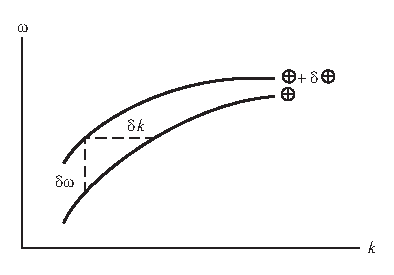
\includegraphics{../figures/chap11/fig22.eps}
\end{center}
\caption[dkdom relation]{\label{11.fig.dkdom}
两个地球模型$\earth$ 和 $\earth+\delta\earth$的频散曲线示意图。
如果在固定波数$k$下频率的微扰$\delta\omega$为正,
那么在固定频率下波数的微扰$\delta k$则为负。
这两个一阶微扰之间的关系是$\delta k=-C^{-1}\delta\omega$,
其中$C=d\omega\hspace{-0.2 mm}/\hspace{-0.2 mm}dk$是扰动前曲线的斜率。
}
\end{figure}

%\subsection{Fr\'{e}chet derivatives of phase speed}
\subsection{相速度的Fr\'{e}chet导数}
\index{phase speed!Fr\'{e}chet derivative of|(}%
\index{Fr\'{e}chet kernel!phase speed|(}%

(\ref{11.threeperts})式使我们能够计算
波数$k$或相速度$c$相对于用来给定球对称地球模型的参数的Fr\'{e}chet导数。
例如,在各向同性模型中,相速度相对于压缩波速度$\alpha$、剪切波速度$\beta$、密度$\rho$
和不连续面半径$d$的Fr\'{e}chet导数可以用(\ref{eq:9.Kkap})--(\ref{eq:9.Kd})
和~(\ref{eq:9.Kalpha})--(\ref{eq:9.Krhop})中的积分核表示为
\eq \label{11.pderiv}
\left(\frac{\p c}{\p\alpha}\right)_{\beta,\rho,d}=
\left(\frac{c^2}{C\om}\right)K_{\alpha},\qquad
\left(\frac{\p c}{\p\beta}\right)_{\alpha,\rho,d}=
\left(\frac{c^2}{C\om}\right)K_{\beta},
\en
\eq \label{11.pderiv2}
\left(\frac{\p c}{\p\hspace{-0.2 mm}\rho}\right)_{\alpha,\beta,d}=
\left(\frac{c^2}{C\om}\right)
K_{\raisebox{0.3 ex}{\scriptsize$\rho$}}^{\prime},\qquad
\left(\frac{\p c}{\p d}\right)_{\alpha,\beta,\rho}=
\left(\frac{c^2}{C\om}\right)K_d,
\en
其中下标表明在微分过程中除了角频率$\omega$外,所有其它保持恒定的变量。
\begin{figure}[!t]
\begin{center}
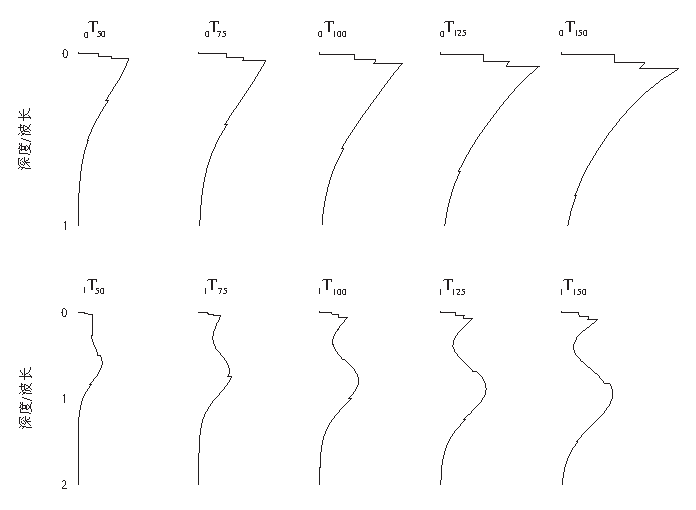
\includegraphics{../figures/chap11/fig23.eps}
\end{center}
\caption[Love kernels]{\label{fig:11.13}
几个等价于基阶({\em 上图\/})和第一个高阶({\em 下图\/})勒夫波模式的Fr\'{e}chet 导数
$(\partial c/\partial\beta)_{\alpha,\rho,d}$
随无量纲化深度$z/\lambda$的变化。
}
\end{figure}
这些$c$、$k$ 和 $\om$的导数的"形状"是相同的,表明
行波或驻波对于在不同深度上地球性质的变化的敏感程度是相同的;
比较~(\ref{11.pderiv})--(\ref{11.pderiv2})与~(\ref{9.pderiv})--(\ref{9.pderiv2})可以看出这三个敏感度积分核只在绝对量级上有所不同。

在图~\ref{fig:11.13} 和~\ref{fig:11.14}中,
我们展示了几个等价于基阶和第一个高阶勒夫和瑞利波模式的Fr\'{e}chet导数$(\p c/\p\alpha)_{\beta,\rho,d}$
和 $(\p c/\p\beta)_{\alpha,\rho,d}$;
在所有例子中,自变量均为深度除以渐近的面波波长,
\eq
\frac{z}{\lambda}=\frac{a-r}{2\pi k^{-1}}.
\en 
\begin{figure}[!t]
\begin{center}
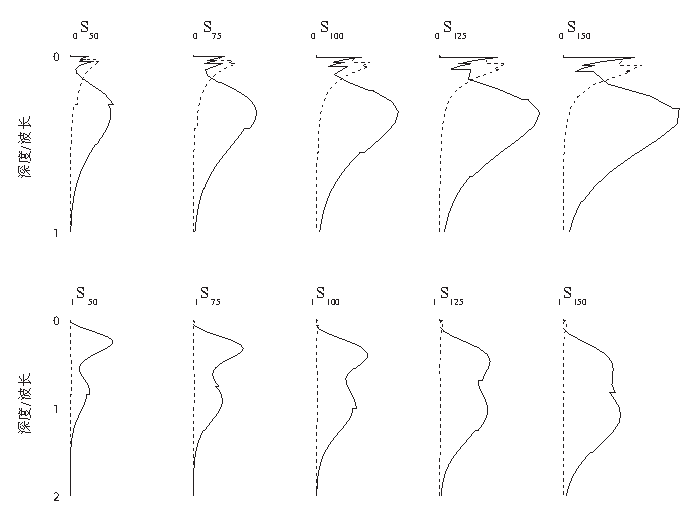
\includegraphics{../figures/chap11/fig24.eps}
\end{center}
\caption[Rayleigh kernels]{
\label{fig:11.14}
几个等价于基阶({\em 上图\/})和第一个高阶({\em 下图\/})瑞利波模式的Fr\'{e}chet 导数
$(\partial c/\partial\alpha)_{\beta,\rho,d}$
({\em 虚线\/})和
$(\partial c/\partial\beta)_{\alpha,\rho,d}$
({\em 实线\/})
随无量纲化深度$z/\lambda$的变化。}
\end{figure}
我们可以看到,用这种无量纲方式缩放后的深度,
在一个给定的面波频散分支上的所有的敏感度积分核看上去完全是一样的!
一个值得牢记的 "经验法则 "是,
基阶的勒夫和瑞利波分别可以"感受"到从地表到约四分之一个和二分之一个波长深度范围内的剪切波速度$\beta$的微扰:
\eq \label{11.skind}
z_{\rm L}\approx\lambda/4,\qquad
z_{\rm R}\approx\lambda/2.
\en
因此,勒夫波比瑞利波能够更强烈地受到岩石圈中剪切波速显著的横向变化的影响。
第一个高阶的勒夫和瑞利波能够极大地改善在深部的分辨率;
\index{surface-wave resolution depth}%
\index{resolution depth}%
它们对于$\beta$微扰的敏感度可以分别延伸到约一个和一个半波长的深度。
这使得在上地幔层析成像反演中加入高阶模式的频散测量或是
由拟合等价的${\rm SS}+{\rm SSS}+\cdots$体波而得到的约束
变得十分有益。
基阶的瑞利波对于浅部的压缩波速度$\alpha$的变化也有有限的敏感度,约到八分之一个波长的深度。
高阶的瑞利波基本上不依赖于$\alpha$。
\index{phase speed!Fr\'{e}chet derivative of|)}%
\index{Fr\'{e}chet kernel!phase speed|)}%

%\subsection{Fr\'{e}chet derivatives of group speed}
\subsection{群速度的Fr\'{e}chet 导数}
\index{group speed!Fr\'{e}chet derivative of|(}%
\index{Fr\'{e}chet kernel!group speed|(}%

模型参数的微扰对群速度的影响可以通过对~(\ref{11.Ccreln})这一关系做Fr\'{e}chet微分而得到。
$C$相对于任一模型参数$m=\alpha,\beta,\rho,d,\ldots$的Fr\'{e}chet导数为
\eq \label{11.LAST}
\frac{\p C}{\p m}=\frac{C}{c}\left(
2-\frac{C}{c}\right)\frac{\p c}{\p m}
+\om\left(\frac{C}{c}\right)^2\frac{\p}{\p\om}
\hspace{-0.5 mm}\left(\frac{\p c}{\p m}\right).
\en
(\ref{11.LAST})式的最后一项可以用相速度敏感度积分核$\p c/\p m$的一阶差分式数值微分来计算
(Rodi, Glover, Li \&
Alexander \citeyear{rodi&al75})。
或者也可以将$\p_{\omega}(\p c/\p m)$用$\p_{\omega}U$、
$\p_{\omega}V$、$\p_{\omega}W$ 和
$\p_{\omega}\phi$这些量来表示,而这些对频率的导数可以通过对本征函数所满足的径向方程和边界条件的微分来计算(Gilbert \citeyear{gilbert76b})。
$(\p c/\p\beta)_{\alpha,\rho,d}$ 和
$(\p C/\p\beta)_{\alpha,\rho,d}$这两个剪切波敏感度积分核在细节上有很大差异;
然而,~(\ref{11.skind})式所表示的基阶勒夫和瑞利波趋肤深度的“经验法则”
\index{skin depth}%
同时适用于群速度和相速度的导数。
\index{group speed!Fr\'{e}chet derivative of|)}%
\index{Fr\'{e}chet kernel!group speed|)}%
\index{surface-wave perturbation theory|)}%
\index{perturbation!surface-wave|)}%

